\documentclass[11pt]{article}
\usepackage{a4wide}

\usepackage[english,dutch]{babel}
% better color management than parallel:
\usepackage{pdfcolparallel}

%\usepackage{parallel}
\usepackage{color}
\usepackage{amsmath}
\usepackage{graphicx}

\usepackage{inconsolata} %a different monofont, texlive-fonts-extra needed!

\usepackage{arduinohighlight}


\usepackage{xcolor}
\usepackage{framed}
\colorlet{shadecolor}{gray!50}

\usepackage[
      %dvipdfm,    %put here the correct(!) driver you are using
      pdftex,
      unicode,
      colorlinks=true,    %no frame around URL
      urlcolor=blue,    %blue color
      menucolor=black,    %no colors
      linkcolor=blue,    %blue color
      bookmarks=true,    %tree-like TOC
      bookmarksopen=true,    %expanded when starting
      hyperfootnotes=false,    %no referencing of footnotes, does not compile
      pdfpagemode=UseOutlines,    %show the bookmarks when starting the pdf viewer
      pdfauthor={Ingegno.be},
      pdftitle={Fe Cube - Ingegno.be},
]{hyperref}


\newtheorem{opdrE}{Task} 
\newenvironment{doE}
  {\begin{shaded}\begin{opdrE}}
  {\end{opdrE}\end{shaded}}

\newtheorem{opdrN}{Opdracht} 
\newenvironment{doN}
  {\begin{shaded}\begin{opdrN}}
  {\end{opdrN}\end{shaded}}
\newtheorem{code}{Code} 

%% First to \eng, then \ned, closes automatically with a paragraph
% \newcommand{\eng}[1]{\selectlanguage{english} \ParallelLText{#1}}
% \newcommand{\ned}[1]{\selectlanguage{dutch} \ParallelRText{#1} \ParallelPar}
% \newcommand{\engt}[1]{{#1} - }
% \newcommand{\nedt}[1]{{#1}}
% \newcommand{\engo}[1]{\eng {#1}}
% \newcommand{\nedo}[1]{\ned {#1}}

%% Use following for book in English language
\newcommand{\eng}[1]{\selectlanguage{english} {#1}}
\newcommand{\ned}[1]{\selectlanguage{dutch} }
\newcommand{\nedt}[1]{ }
\newcommand{\engt}[1]{{#1}}
\newcommand{\nedo}[1]{\selectlanguage{dutch} }
\newcommand{\engo}[1]{\selectlanguage{english} {#1}}

%% Use following for book in Dutch language
%\usepackage{multicol}
%\newcommand{\eng}[1]{\selectlanguage{english} }
%\newcommand{\ned}[1]{\begin{multicols}{2}{\selectlanguage{dutch} {#1}}\end{multicols}}
%\newcommand{\engt}[1]{ }
%\newcommand{\nedt}[1]{{#1}}
%\newcommand{\engo}[1]{\selectlanguage{english} }
%\newcommand{\nedo}[1]{\selectlanguage{dutch} {#1}}

%\selectlanguage{english}
% \ParallelLText{\blindtext}
%\selectlanguage{dutch}
%\ParallelRText{\blindtext}
%\ParallelPar


\begin{document}


 \title{Fe Cube: Make it! Understand it!}
 \author{Ingegno Team: M.C. Ciocci, B. Malengier}
 \date{\today}
 \maketitle

\begin{Parallel}{7.5cm}{7.5cm}
 \section{\engt{Introduction} \nedt{Introductie}}
\eng{In this booklet we will show how to create the Fe Cube. You will learn about LEDs, the arduino, multiplexing, soldering, color theory, and more! You can buy a kit from Ingegno.be, or buy your components somewhere else.

The code of this manual can be found on \href{https://github.com/ingegno/linefollower1}{the Ingegno github page}.
}

\ned{In dit boekje zullen we je leren hoe je de Fe Cube kunt maken. Je zal leren over LEDs, de arduino, multiplexing, solderen, kleurentheorie, en meer! Je kan een kit kopen met alle onderdelen van Ingegno.be, of je kan je eigen stukken gebruiken.


De code van deze handleiding kan gevonden worden op \href{https://github.com/ingegno/linefollower1}{de Ingegno github pagina}.
}

\subsection{\engt{The components} \nedt{De componenten}}
\eng{We will need following components: 
\begin{enumerate}
 \item A breadboard
 \item 9 RGB-LED + 3 extra (we assume common kathode for the cube)
 \item 1 big RGB-LED (we assume common anode)
 \item 3 NPN + 1 extra (2N3904 normally)
 \item 9 220 $\Omega$ resistors + 3 extra
 \item many wires
 \item lasercut base for the cube
 \item iron wire pillars for the cube
 \item soldering plate for fixed components + connecter parts
\end{enumerate}
You will also need a soldering iron, and optionally you can make a cover for the cube, eg using 3D printing.

For an overview of meaning of the components, see the cheat sheet distributed seperately.
}

\ned{We zullen volgende componenten gebruiken: 
\begin{enumerate}
 \item Een schakelbord
 \item 9 RGB-LED + 3 extra (we veronderstellen gemeenschappelijke kathode voor de kubus)
 \item 1 grote RGB-LED (we veronderstellen gemeenschappelijke anode)
 \item 3 NPN + 1 extra (2N3904 normaal)
 \item 9 220 $\Omega$ weerstanden + 3 extra
 \item veel draden
 \item lasercut basis voor de kubus
 \item ijzerdraad pilaren voor de kubus
 \item soldering plaat voor vaste componenten + connectiestukken
\end{enumerate}
Je zal ook een soldeerijzer nodig hebben, en optioneel kun je een bedekking maken voor de kubus, bv via 3D printen.

Voor een overzicht van de betekenis van de componenten, zie het overzicht die je apart gekregen hebt.
}

\subsection{Arduino}
\eng{We will make intensive use of Arduino, so you need to install the \href{http://arduino.cc}{Arduino software}. Once installed, you can connect the Arduino to your PC via de usb port.  In the programming environment you installed you can write programs, and load those on the Arduino board. They will be executed there as long as the Arduino recieves power.

}
\ned{We zullen intensief gebruik maken van Arduino, dus moet je de \href{http://arduino.cc}{Arduino software} installeren op je laptop.
Eenmaal geinstalleerd kun je nu je arduino koppelen aan je computer via de usb poort. In de programmeeromgeving van Arduino kun je programma's schrijven en die opladen naar de arduino, waar ze dan uitgevoerd worden zolang er stroom is.
}


\subsection{\engt{Programming with Arduino} \nedt{Programmeren met Arduino}}
\eng{A programming language needs to be understood by a computer. Unfortunately computers are still a little bit dumb, so you are not allowed to make errors! It's like a writing contest in which you need to obtain a 10/10 every time. So take time to learn the form of the language. See the specific sheet 'programming with arduino' distributed with this manual.}


\ned{Een programmeertaal moet verstaan worden door een computer. Spijtig genoeg zijn computers nog altijd een beetje dom, dus mag je geen enkele fout maken! Het is zoals een dictee waar je altijd 10/10 moet halen. Neem dus de tijd om de structuur en taal van de Arduino te leren. Zie de blaadjes 'Programmeren met Arduino' die je bij deze gids kan downloaden.}

\section{\engt{Lesson 1: One Led Circuit} \nedt{Les 1: \'E\'en Led circuit}}
\eng{We will make a circuit with one LED, which we will program to blink. The Arduino outputs 5 Volt, while the Led are designed for 3 Volt. Hence we will use a resistor to reduce the voltage over the Led. For Led, the resistor is best on the anode side (= the + side, which corresponds to the longest leg of the LED). You can calculate the resistor you need with \url{http://led.linear1.org/1led.wiz}}.

\subsection{\engt{One pin} \nedt{\'E\'en pin}}
\eng{Make the circuit as indicated in Fig.~\ref{f:lesson1_onepin}. Use your breadboard and wires to make the connections. A wire from pin 2 to row 10 on the breadboard. Then the resistor of R=330 $\Omega$ from row 10 to row 6, the LED anode from row 6 to row 5, and finally a wire from row 5 to the GND pin on the Arduino. You can see }
\ned{Maak het circuit zoals gegeven in Fig.~\ref{f:lesson1_onepin}. Gebruik je schakelbord en draden om de connecties te maken. dus hier, een draad van pin 2 naar rij 10 op je schakelbord. Dan de resistor met weerstand R=330 $\Omega$  van rij 10 naar rij 6, de LED anode van rij 6 naar rij 5, en uiteindelijk een draad van rij 5 naar de GND pin op de Arduino.}

\begin{figure}
  \centering
  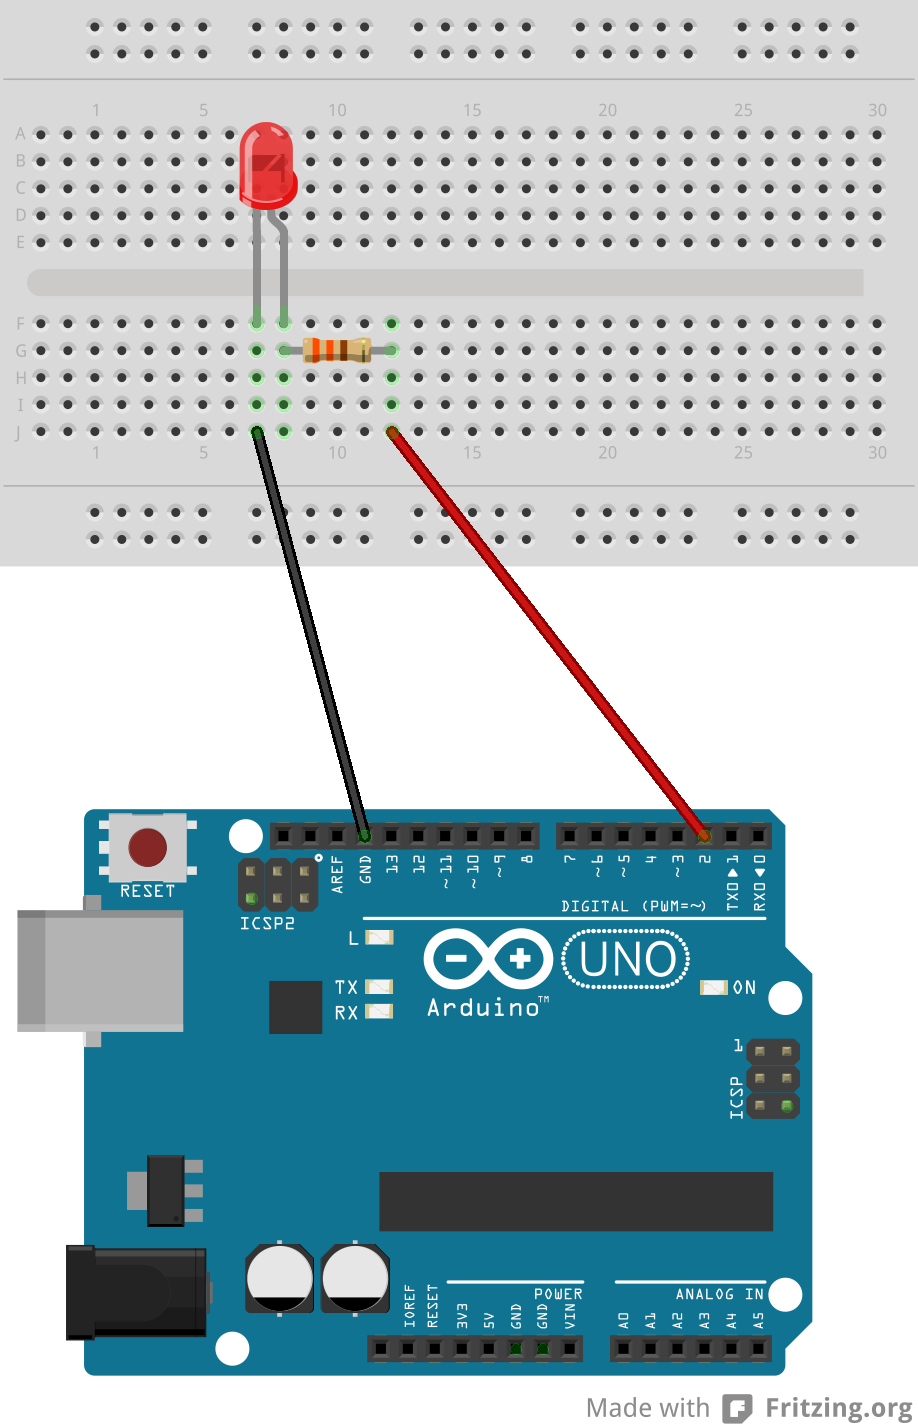
\includegraphics[width=6cm]{img/01_onepin_oneled_bb}\ \ 
   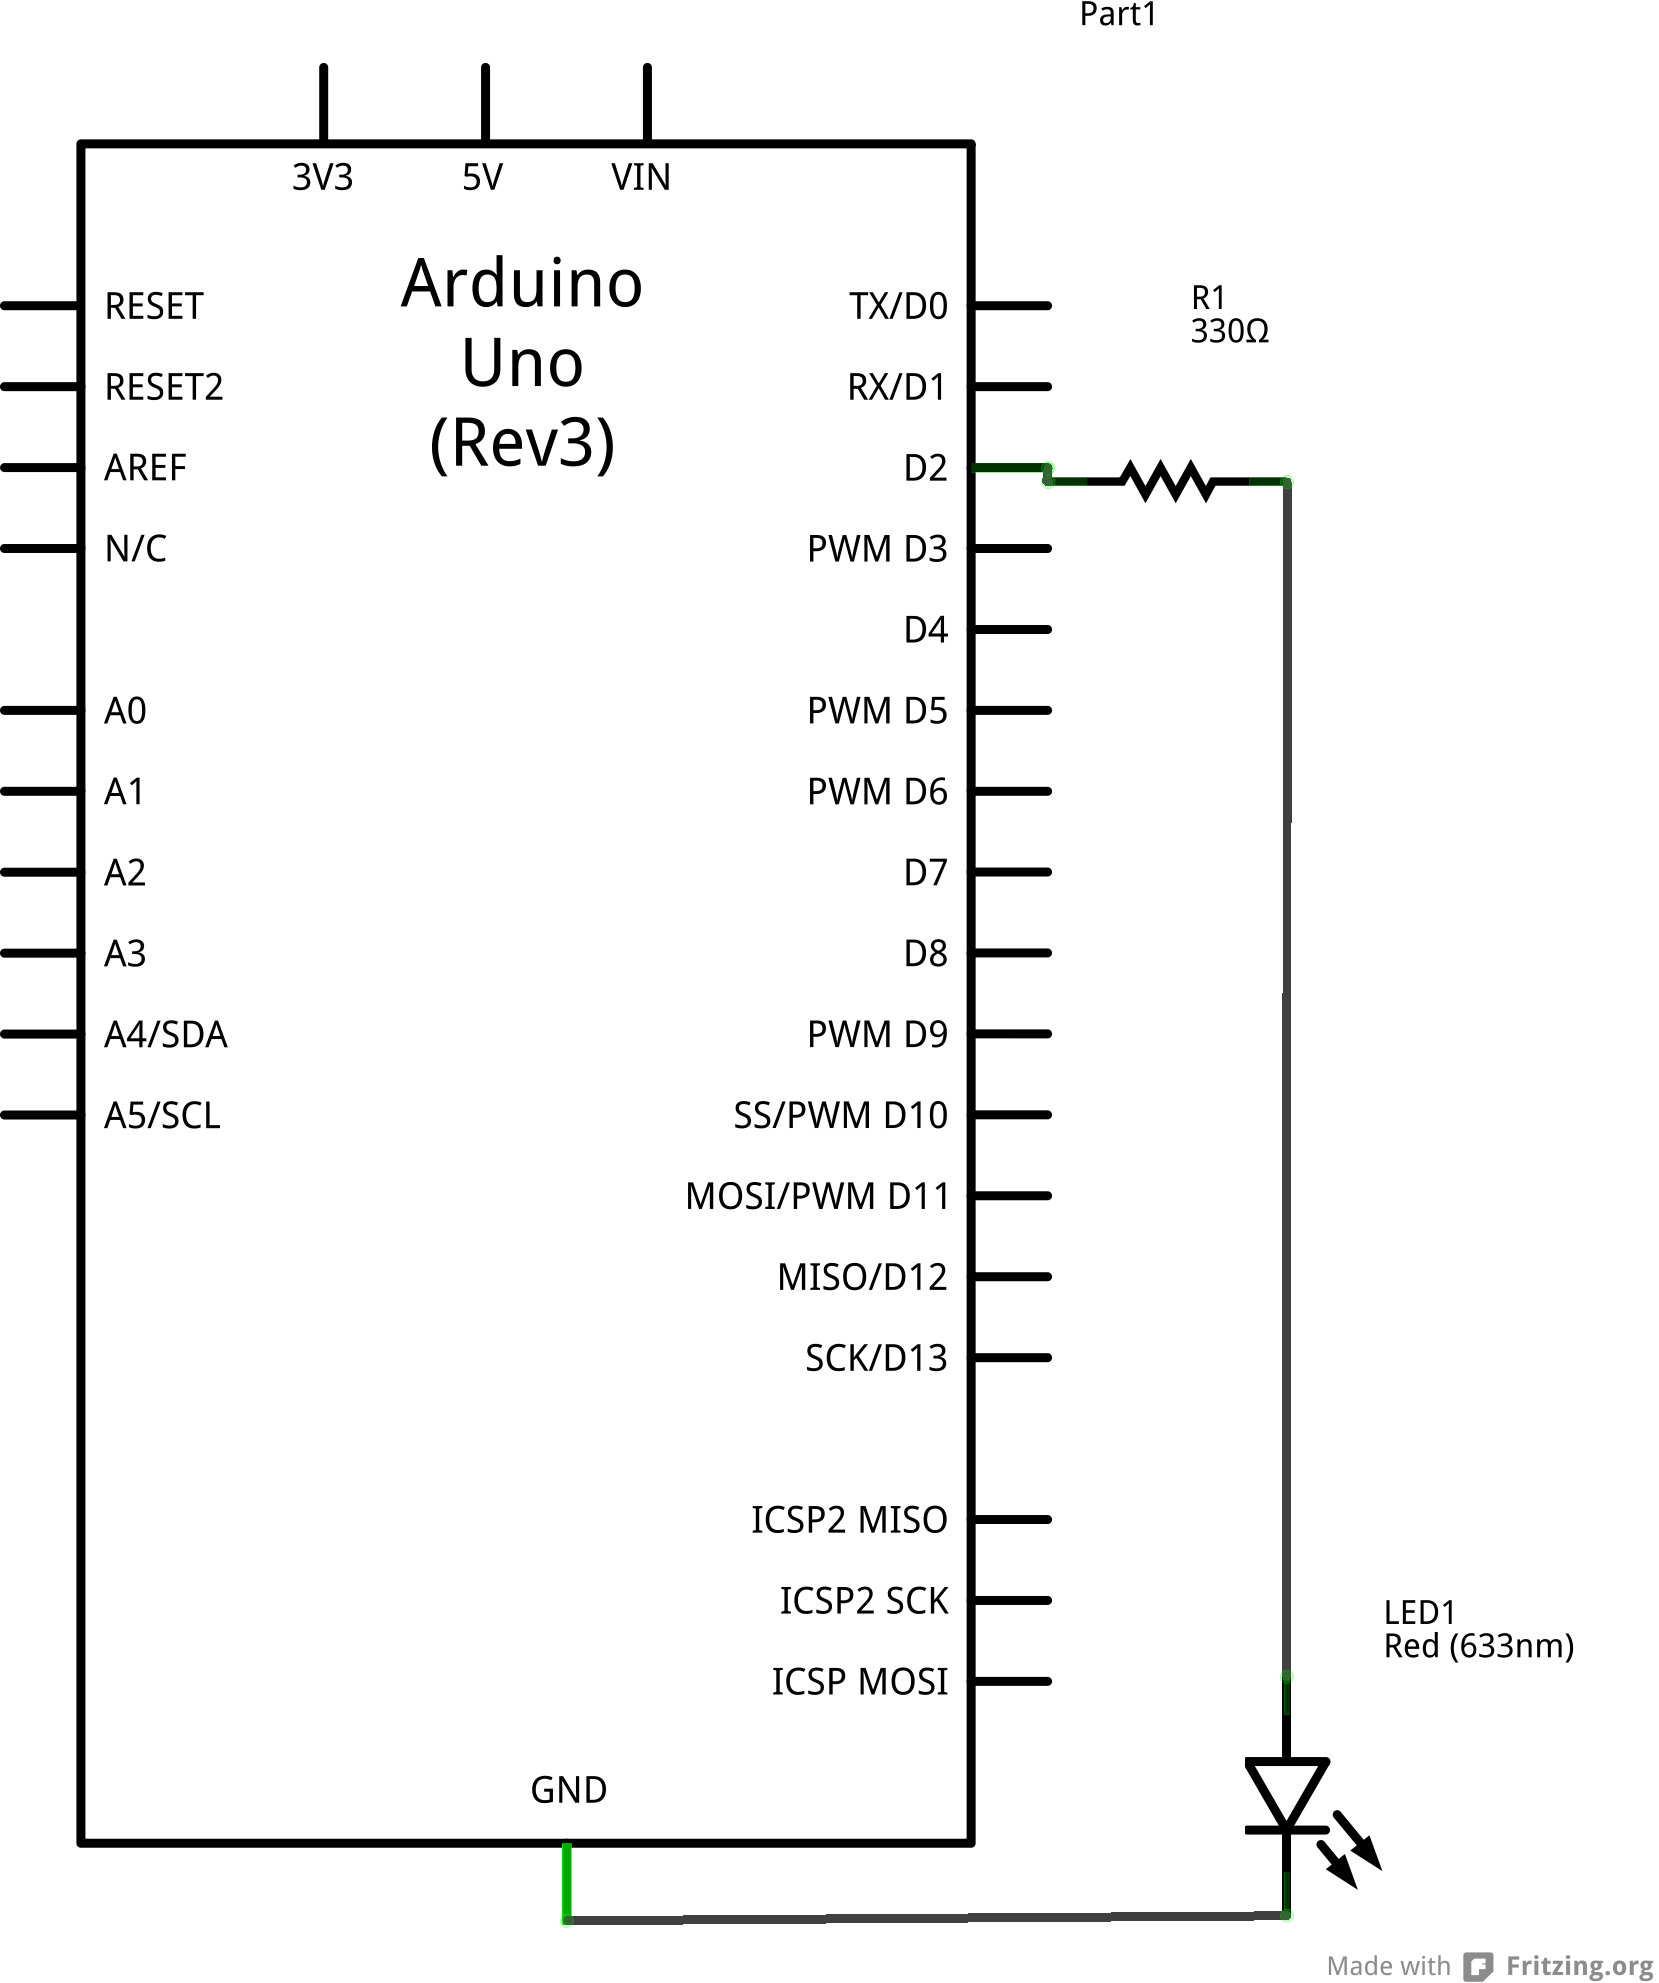
\includegraphics[width=6cm]{img/01_onepin_oneled_schem} 
\caption{\engt{Using one pin and the ground, we can make a LED burn. Left with breadboard, right as a schematic}
\nedt{Met een pin en de grond kunnen we een LED doen branden. Links met breadboard, rechts als schema.}}
\label{f:lesson1_onepin}       % Give a unique label
\end{figure}

\eng{We now need to write a program that sets the power to pin 2 on and off every second, so that the LED blinks. You see the code in Code \ref{c:l1_a}.}
\ned{Nu moeten we een programma schrijven dat de stroom naar pin 2 aan en af zet elke seconde, zodat de LED pinkt. Je vindt de code in Code \ref{c:l1_a}.}

\begin{code}\label{c:l1_a}
 \ \newline
\inputardfull{\string"../sketches/Fe_cube_01_led_one_pin/Fe_cube_01_led_one_pin.ino\string"}
\end{code}

\engo{\begin{doE}
      Congratulations, you made your first programmable Led. Change the program so that the led blinks every 3 seconds, with 1 second off. Next, what does it happen if you blink every 40 milliseconds and every 10 milliseconds?
     \end{doE}
}
\nedo{\begin{doN}
      Proficiat, je hebt je eerste programmeerbare led gemaakt. Verander nu je programma zodat de led elke 3 seconden pinkt, met 1 seconde af. Vervolgens, wat gebeurt er als je elke 40 milliseconden pinkt en als het elke 10 milliseconden pinkt? 
     \end{doN}
}
\eng{How does it work? Well, the pins from 1 to 13 can have a HIGH state or a LOW state. HIGH means the pin has 5V of power, while LOW means the pin is in the ground state GND. We say that current flows from the positive voltage of 5V (the + side) to the GND (the - side). This is somewhat annoying as the actual quantum particles used here, called electrons, actually go the other way. So, they flow from the minus to the plus. This because they have themself a negative charge, so they are repelled by the negative GND. Theoretically you could use other quantum particles however! Anyway, the direction of the current, from + to - is just an agreement between scientists. 

The power source here is 5V, which is an indication of how much work you can do. A lot of power means you do a lot of work! To burn a LED we don't need a lot of power however, so we reduce the power used to burn the LED by adding a resistor. This increases the lifetime of the LED.

The resistor is just that, it resists the flow of the current, and hence the quantum particles loose some of their power going through the resistor. Not only will the particles have less power however, there will also be less particles that can pass the resistor every second, or in other words, the current is also lower. So a resistor will decrease the current, and after passing it there is also less power left to do the rest of the circuit. 

Next comes the LED for the current. All the remaining power will be used to go through the LED and generate light. A LED only produces light if the anode (long leg, +) is connected to the voltage (positive side), and the cathode (short leg) towards the GND side. If you put the LED around (try it!) there will be no light. There will also be very little current going through the LED in this way because not only does it produce no light, it will also resist the current a lot if the anode is connected to the GND. A blow up of a LED is shown in Figure \ref{f:LED}.}


\ned{Hoe werkt ons circuit? Wel, de pinnen van 1 tot 13 kunnen een HIGH staat en een LOW staat hebben. HIGH betekent dat de pin 5V krachtbron heeft, terwijl LOW betekent dat de pin zich in de grond staat bevindt. We zeggen dat stroom sroomt van de positieve voltage van 5V (de + zijde) naar de GND (de - zijde). dat is een beetje vervelend gezien de echte kwantumdeeltjes die hier gebruikt worden, electronen genoemd, eigenlijk de andere kant op stromen, dus van de min naar de plus. Dit omdat elektronen zelf negatief zijn, en dus afgestoten worden door de negatieve lading van de GND. Theoretisch zou je evenwel andere kwantumdeeltjes kunnen gebruiken! Hoe dan ook, de richting van de stroom, van + naar -, is gewoon een afspraak tussen wetenschappers om geen verwarring te doen ontstaan. 

De krachtbron is hier 5 Volt (5V), wat een indicatie is van hoeveel werk je kan doen. Veel kracht betekent dat je veel werk kan doen! Om een LED te doen branden hebben we evenwel niet veel kracht nodig, dus beperken we die door een resistor toe te voegen die de kracht over de LED zal beperken. Dit verhoogt de levensduur van de LED.

De resistor of weerstand is effectief wat het zegt: het resisteert of weerstaat de stroom. Bijgevolg verliezen de kwantumdeeltjes een deel van hun kracht als ze door een weerstand stromen. Niet alleen zullen de deeltjes minder kracht hebben erna, er zullen ook minder deeltjes passeren elke seconde. De stroom is dus verminderd. Een weerstand of resistor zal dus de stroom verminderen en na het passeren zal er ook nog eens minder kracht over zijn om door de rest van het circuit te stromen.

Daarna komt de LED voor de stroom. Alle overblijvende kracht zal gebruikt worden om door de LED te gaan en licht te genereren. Een LED maakt alleen licht als de anode (lange been, +) is geconnecteerd naar het votage (de positieve zijde), en de kathode (korte been, -) naar de GND zijde.
Als je de LED ronddraait (probeer het!) zal er geen licht schijnen. Er zal ook maar heel weinig stroom vloeien dan, gezien de LED niet enkel geen licht maakt dan maar ook de stroom sterk zal weerstaan. Een LED in het groot zie je in Figuur \ref{f:LED}.
} 


\begin{figure}
  \centering
  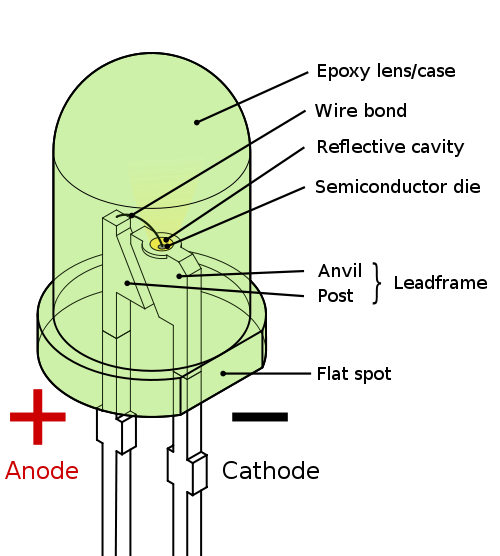
\includegraphics[width=6cm]{png/LED}
\caption{\engt{Blow up view of a LED}
\nedt{Een LED in het groot}}
\label{f:LED}       % Give a unique label
\end{figure}


\engo{\begin{doE}
      Study the schematic to the right of Figure \ref{f:lesson1_onepin}. A schematic is often more clear to work with than the wires drawn to the left. Every component has it's own symbol. For example, the LED is a triangle ending on a short vertical line, and two small arrows indicating the light that is emitted. The triangle in this symbol can be interpreted as an arrow indicating the direction of the current: from + to -. The light leaves the LED in the same direction.
     \end{doE}
}
\nedo{\begin{doN}
      Bestudeer het schema aan de rechterkant van Figuur  \ref{f:lesson1_onepin}. Een schema is vaak duidelijker om mee te werken dan de draden die je aan de linkerkant ziet. Elke component heeft zijn eigen symbool. Een LED is een driehoek die eindigt op een korte vertikale lijn, en twee kleine pijlen die het licht voorstellen die de LED uitzendt. De driehoek in dit symbool kun je interpreteren als een grote pijl die de richting van de stroom aanduidt: van + naar -. Het licht verlaat de LED in dezelfde richting in het symbool.
     \end{doN}
}

\eng{You want to know how the LED produces light? Well, that is quantum physics, something most people never learn. Let's explain a bit. To understand quantum physics, you need to work with the quantum particles, so here electrons. Remember, the electrons go from GND to the pin 2, so from the cathode (-) to the anode (+) of the LED. 

At the cathode side, the LED has what is called an n-type material. This is a material that has an excess in negative electrons, hence n. At the anode side there is a p-type material. This material has a shortage of electrons, which we call holes: it is the absense of an electron within the material. The p-type material passes current by moving holes around. The n-type material by moving electrons around. 

So, if electrons arrive at the cathode, they create a surplus of electrons, and the electrons are pushed towards the p-type material. There, they fall into a hole, and this is a quantumeffect that creates a small quantum of energy, which is a photon, and which we see here as the light of the LED. This effect is called \textit{Electroluminescence}, and only happens from an n-type material to a p-type material. Between other materials that transport electrons, the electrons can loose energy gradually, instead of in quanta. 

Now, after this drop, there are less holes in the p-type material in the direction of the n-type material, so the holes in the p-type material move towards this place so as to rebalance the amount of holes. The resulting shortage of holes at the cathode side then causes an electron to leave the p-type material entirely (the material likes it's amount of holes and wants to keep it like that), creating a new hole there.

If you switch the LED around, you connect the n-type material to the positive voltage. The electrons of the n-type material then just flow towards this voltage creating too little electrons in the material. This can only be corrected by an electron leaving the p-type material and like that creating a new hole there and a new electron in the n-type material. However, this clearly does not produce light (as the electron does not fall into a hole), but the electrons also resist a lot against moving from the p-type material to the n-type material (they are comfortable where they are and resist jumping, or seen differently, the material likes it's amount of holes and tries to keep it like that.). 
}
\ned{Je wil weten hoe de LED licht produceert? Wel, dat is kwantumfysica, en de meeste mensen leren daar nooit over. Laat ons het een beetje uitleggen. Om kwantumfysica te verstaan moet je met kwantumdeeltjes werken, dus hier de elektronen. Herinner, de elektronen stromen van de GND naar de pin 2, dus van de kathode (-) naar de anode (+) van de LED. 

Aan de kathode zijde zit wat we een n-type materiaal noemen. Dit is een materiaal die een overschot aan negatieve electronen heeft, daarom n. Aan de anode zijde zit een p-type materiaal. Dat is een materiaal die een tekort aan elektronen heeft, wat we gaten noemen: het is de afwezigheid van een elektron in het materiaal. Het p-type materiaal laat stroom door door gaten rond te bewegen. Het n-type materiaal door elektronen rond te bewegen.

Dus, als elektronen toekomen aan de kathode cre\"eren ze daar een surplus aan elektronen, en de elektronen worden geduwd in de richting van het p-materiaal. Daar aangekomen vallen ze in een van de gaten, en het is dit kwantumeffect dat een klein kwantum aan energie cre\"eert, welke een foton is wat we zien als het licht van de LED. Dit effect noemen we  \textit{Electroluminescentie}, en het gebeurt enkel bij overgang van een elekrton van een  n-type materiaal naar een p-type materiaal. Tussen andere materialen die elektronen doorlaten kunnen de elektronen altijd gradueel hun energie verliezen, in plaats van via een kwantum. 

Nu, na het vallen in het gat zijn er minder gaten in het p-type materiaal aan de kant van het n-type materiaal, dus zullen de gaten bewegen in die richting om terug een gelijke balans in het materiaal te hebben. Hierdoor eindigen we met een tekort aan gaten aan de kathode zijde, welke op zijn beurt ervoor zal zorgen dat een elektron het materiaal zal verlaten (het materiaal houdt van zijn aantal gaten en wil het zo houden), waardoor een nieuw gat ontstaat daar.

Als je de LED omdraait, connecteer je het n-type materiaal aan de positieve krachtbron. De elektronen van het n-type materiaal stromen dan gewoon naar deze krachtbron, zo een tekort aan elektronen veroorzakend daar. Dit kan enkel gecorrigeerd worden door een elektron dat het p-type materiaal verlaat, en zo een nieuw gat cre\"eert, en een nieuw elektron in het n-type materiaal. Dit evenwel zal duidelijk geen licht produceren (gezien het elektron niet in een gat valt), maar de elektronen bieden ook heel veel weerstand in het bewegen van het p-type materiaal naar het n-type materiaal (ze zijn bij wijze van spreken comfortabel waar ze zijn, het materiaal houdt van zijn aantal gaten en wil het zo houden).
}
\begin{figure}
  \centering
  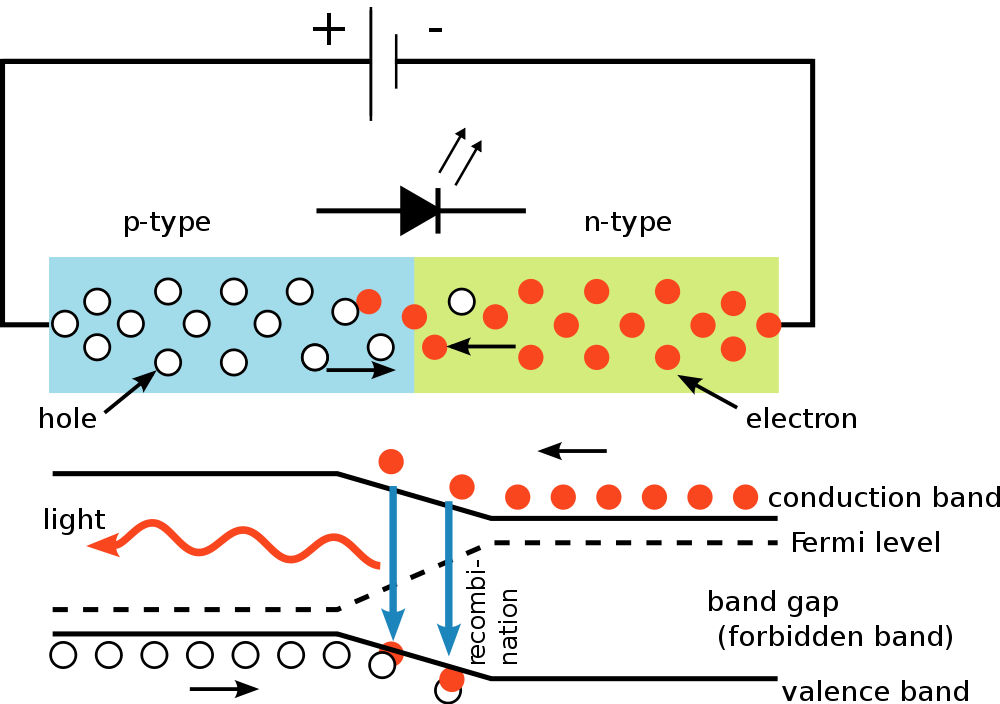
\includegraphics[width=10cm]{png/PnJunction-LED}
\caption{\engt{A PN junction as used in a LED}
\nedt{Een PN overgang zoals gebruikt in een LED} (\textcopyright Wikimedia Commons S-kei)}
\label{f:NPJunction}       % Give a unique label
\end{figure}

\subsection{\engt{Adding NPN, two pins} \nedt{Nu met NPN, twee pinnen}}
\eng{Controlling the LED worked great, but we will later need the ability to cut off the power on the Cathode (-) side too, so towards the ground (GND). In this section we will learn how to do that. One possibility is to use a switch: a component that is on and off depending on a signal. Just like the light switches you use every day and where the input is the press of your hand touching it. We will use the smallest switch possible: an NPN gate. This piece is the half cilindrical black piece with 3 legs in your box, see Fig.~\ref{f:Tr_Pinouts}. 
}



\ned{De LED controleren werkte perfect, maar later zullen we de mogelijkheid willen om de stroom af te sluiten aan de Kathode zijde (-), dus aan de grond (GND). In deze sectie zullen we dat leren. Een mogelijkheid is om een schakelaar te gebruiken: een component die aan of af is afhankelijk van een signaal. Net zoals de lichtschakelaars die je dagelijks gebruikt, en waar de input de druk van je hand is. We zullen de kleinst mogelijke schakelaar gebruiken: een NPN brug. Dit stuk is de halve zwarte cilinder met 3 poten in je doos, zie Fig.~\ref{f:Tr_Pinouts}. 
}


\begin{figure}
  \centering
  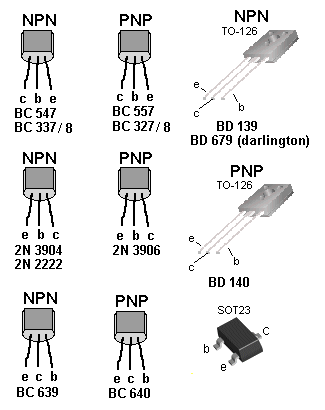
\includegraphics[width=6cm]{png/Tr-Pinouts} 
\caption{\engt{Different NPN and PNP transistors. There is no standard for the pinouts, so use a datasheet, or try it with a LED like we do. If it does not work, use other legs as in this Picture!}
\nedt{Verschillende NPN en PNP transistoren. Er is geen standaard voor de beentjes, refereer naar een datasheet, of probeer het met een LED zoals wij hier doen. Als het niet werkt, gebruik andere beentjes zoals in deze Figuur!}}
\label{f:Tr_Pinouts}       % Give a unique label
\end{figure}

\eng{As you can see in that figure, there is no standard for identifying the legs of the transistor. Normally, the one you have will have, looking at the flat side of NPN, the left leg as the in-side for the current (C, from collector), the right leg is the out-side (E, from extruder/emitter) that goes to the GND, and the middle leg is the P or positive control (B, from the word base). If there is positive power on the P, the NPN gate is open and current can flow to the ground state. If there is no power on the P, the NPN gate is closed. Our complete circuit is then given in Fig.~\ref{f:lesson1_twopin}}

\ned{Zoals je in die figuur ziet is er geen standaard om de beentjes van een transistor te identifici\"eren. Normaal zal het als volgt zijn voor degene die jij zult gebruiken: hou je het rechtop en kijk je naar het vlakke stuk van de NPN, dan is de linkerpoot de in-zijde voor de stroom (C, van collector, waar er gecollecteerd wordt), de rechterpoot de uitgangzijde (E, van extruder) die naar de GND gaat, en het middelste been is de P of positieve controle (B, van basis). Als er een positieve stroom is op P, laat de NPN brug stroom door. Is er geen stroom op de P, dan kan er geen stroom door en is het circuit dus onderbroken. Het complete circuit is gegeven in Fig.~\ref{f:lesson1_twopin}.
}


\begin{figure}
  \centering
  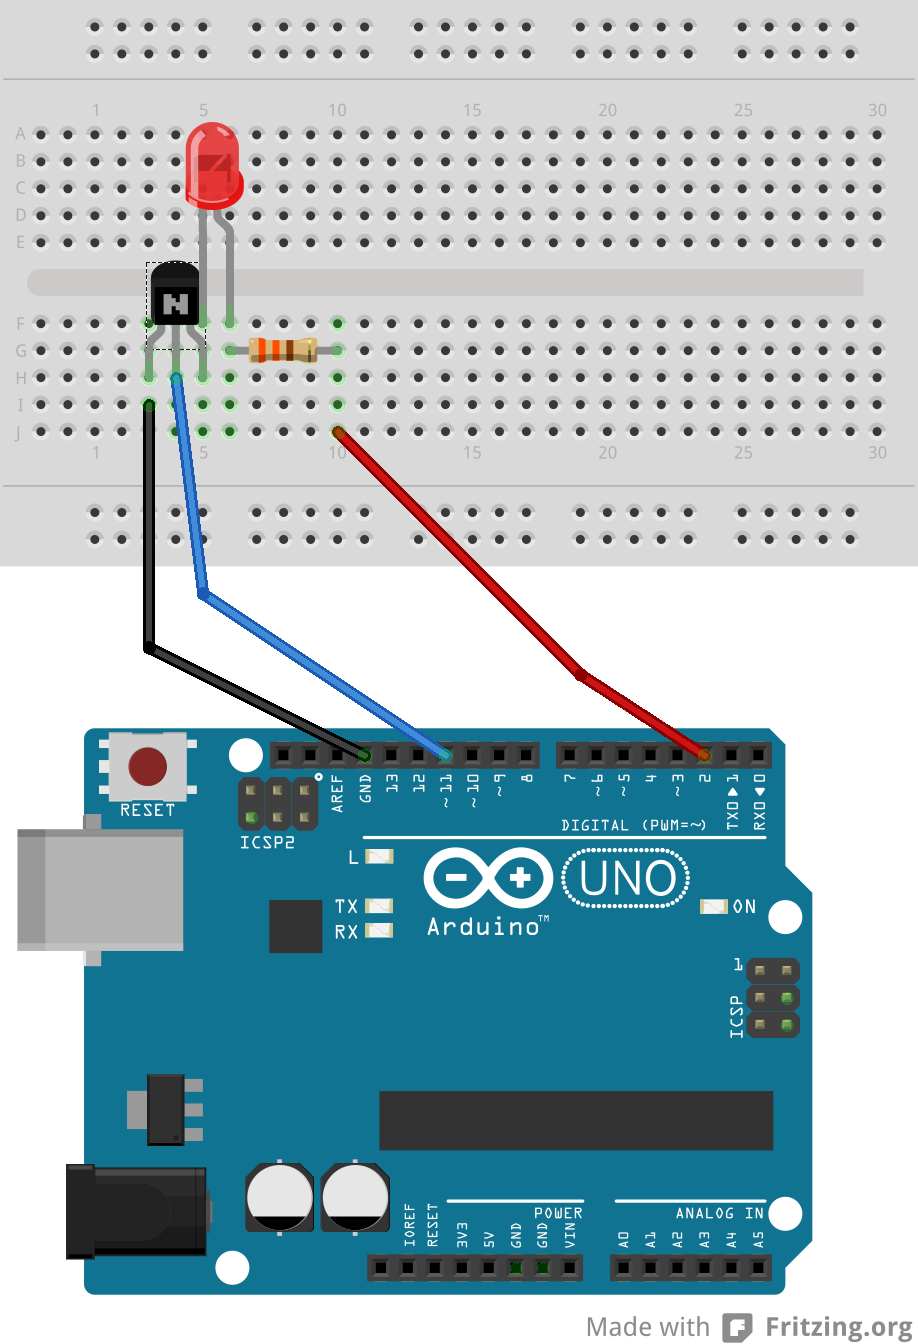
\includegraphics[width=6cm]{img/02_twopin_oneled_npn_bb} \ \ 
  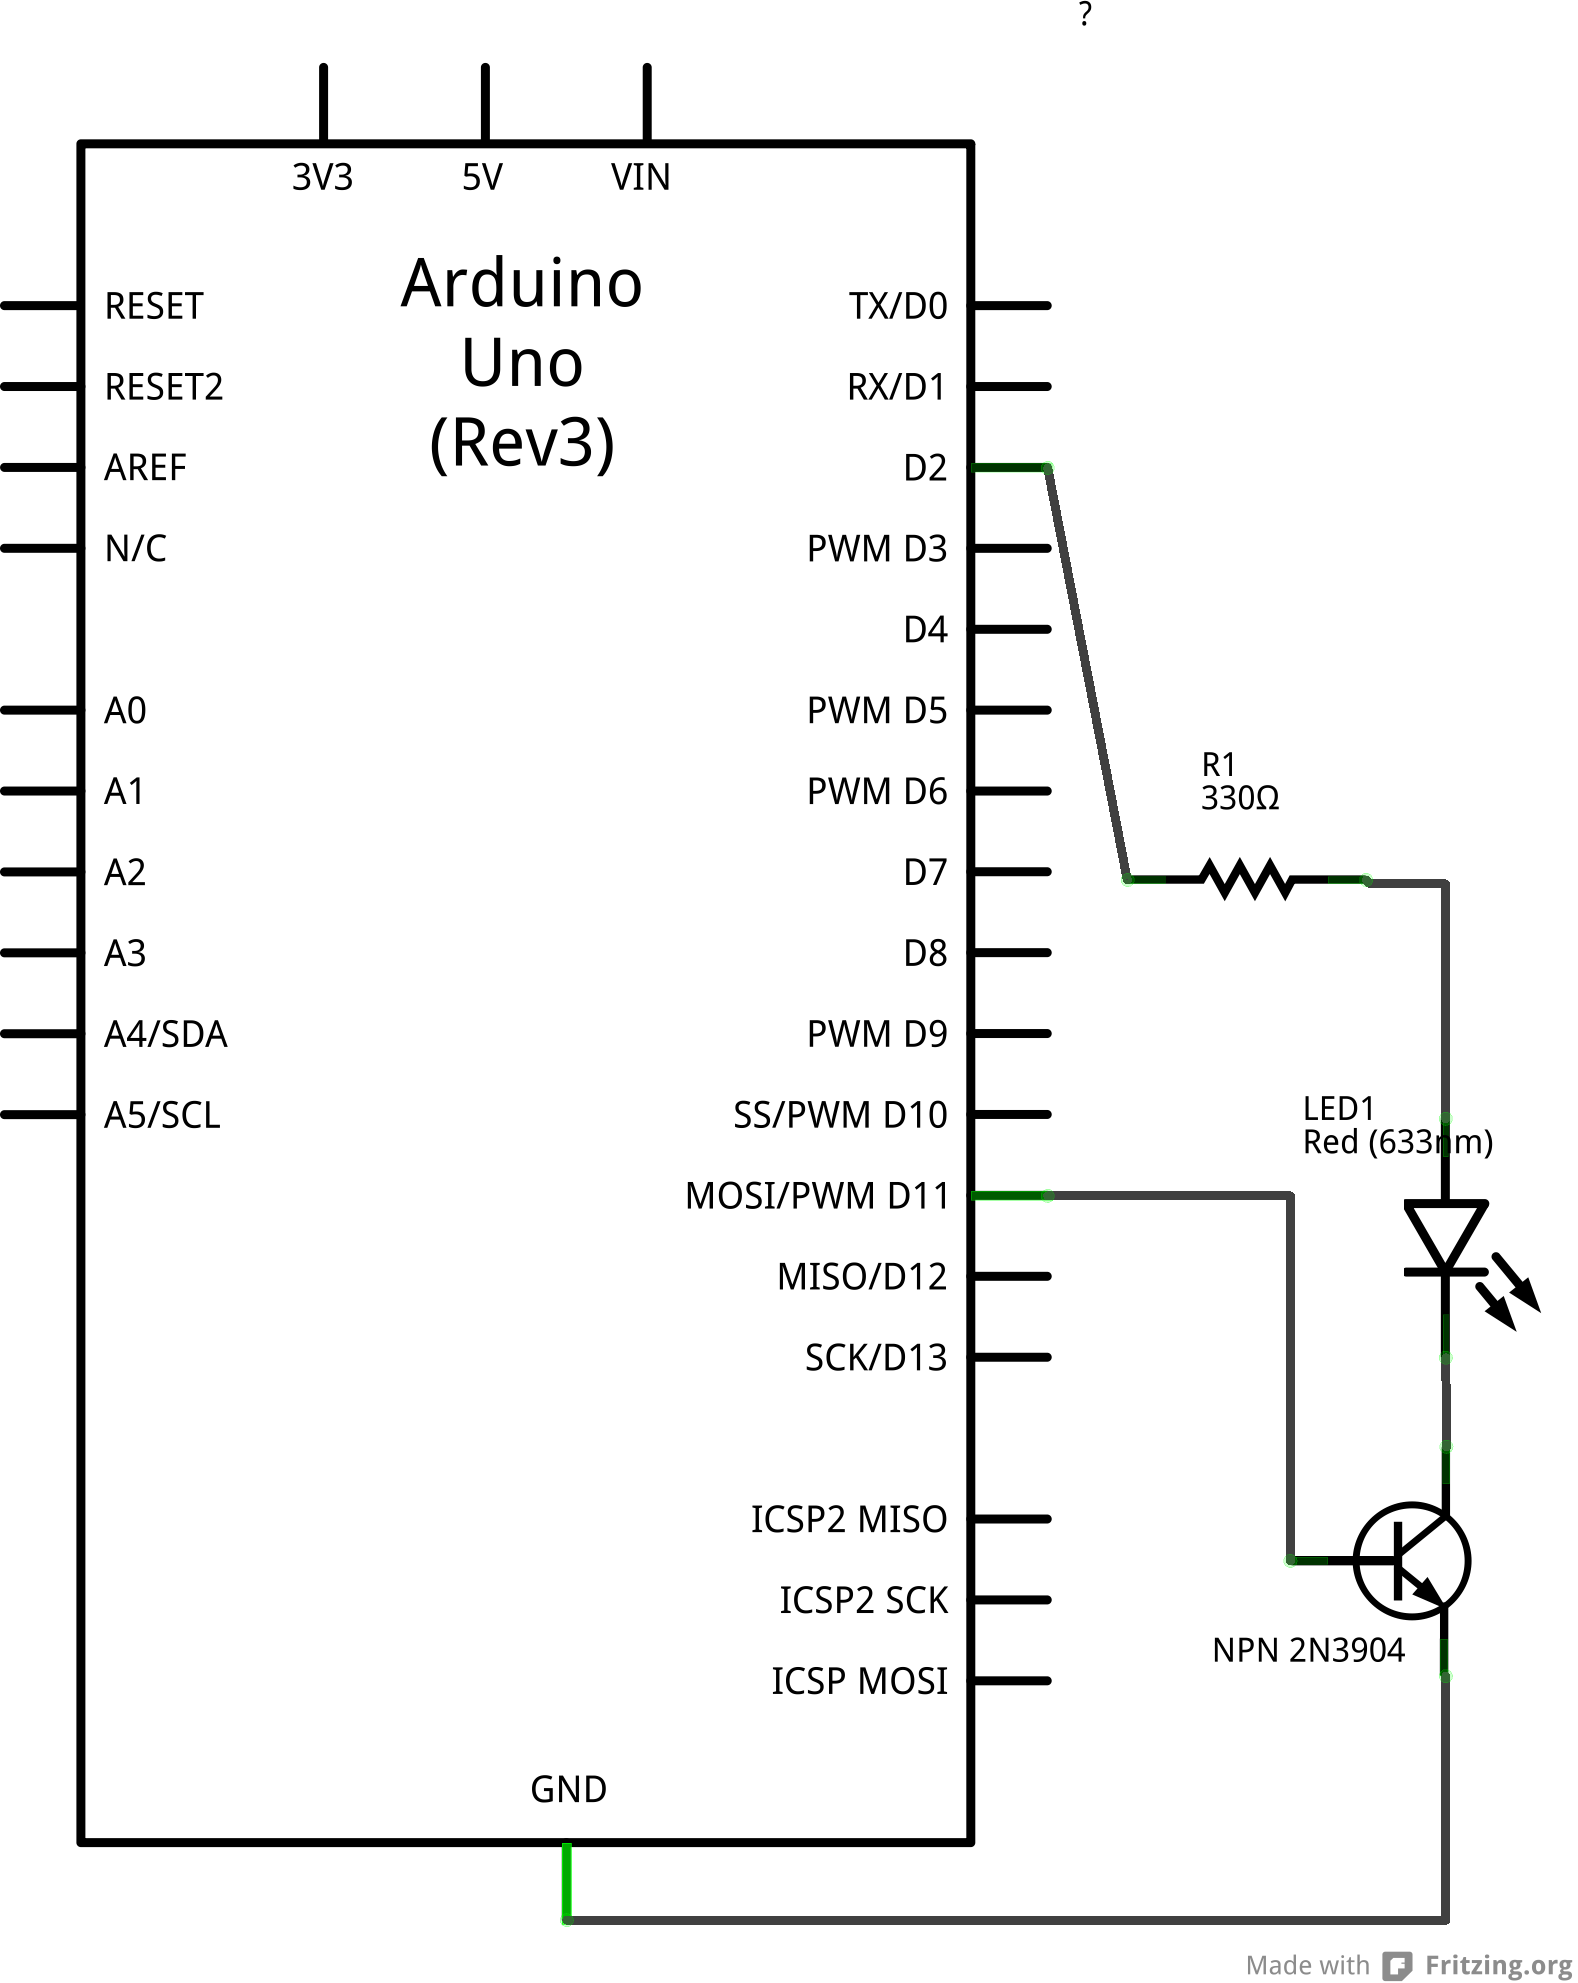
\includegraphics[width=6cm]{img/02_twopin_oneled_npn_schem}
\caption{\engt{Using two pins and an NPN gate, we can switch off the LED on both sides}
\nedt{Met twee pinnen en een NPN brug kunnen we de LED afzetten aan beide kanten.}}
\label{f:lesson1_twopin}       % Give a unique label
\end{figure}


\eng{We now adapt our program so that the pin to the NPN is used to control the LED and make it blink. To see that the NPN works as expected, we cycle the LED through three states each for a second: both arduino pins on; only anode pin on, and only pin to NPN on. Correct behavior means this will result in a LED on for a second, and off for two seconds.}
\ned{Nu moeten we ons programma aanpassen zodat ook de pin naar de NPN gebruikt wordt om de LED te doen blinken. Om vast te stellen dat de NPN werkt zoals verwacht laten we de LED door drie standen gaan, elk voor een seconde: Beide arduino pinnen aan, enkel de anode pin aan, en dan enkel de pin naar de NPN aan. Correct gedrag zou dan moeten zijn dat de LED aan is voor een seconde en af voor twee seconden.}

\begin{code}\label{c:l1_b}
 \ \newline
\inputardfull{\string"../sketches/Fe_cube_01_led_npn/Fe_cube_01_led_npn.ino\string"}
\end{code}


\eng{You would like to know how the NPN works? Well, this is a transistor, we refer to it as a bipolar junction transistor. The LED we explained before is a PN junction. Our NPN indeed consists now of 3 materials that have been connected: An n-type material, a p-type material, and then again an n-type material. This time, the p-type material has only little holes. If we connect it to GND (-), there will even be less holes. As we explained before, a p-type material conducts current with holes, so no current can flow then, and the junction is closed.

If we put a voltage over the p-type material, the material loses it's electrons, and obtains more holes. This means we can have now current from the p-material which is the base, to the emmitter n-material, which is just the same as in our PN junction in the LED. So, the emitter 'emits' our electrons into the base.

So, how to we obtain current from the n-type material, to the n-type material? This should not be possible! The trick is that the p-type material when connected to voltage (+) obtains extra holes, and it can form a line of holes from the emittor n-type material to the collector n-type material. Now something extraordinary happens: the electrons can jump from hole to hole via this line from the emittor to the collector. Moreover, they can do that much, much faster than the holes themself move. In other words, we have an amplification of the current at the base, see Fig.~\ref{f:NPNactive}. If we increase the current in the base, more holes flow in the p-type material, and hence more lines start to connect the emittor with the collector. We can hence convert a small signal at the base into a large signal over the NPN.

Note that we put in our test circuit a 5V signal over the base, which in itself is sufficient to power the LED. Because of this, our base current is actually sufficient to power the LED. This is not a problem, just something to be aware of.
}

\ned{Je zou graag weten hoe de NPN werkt? Wel, dit is een transistor, specifiek een Bipolaire transistor. De LED die we hiervoor gezien hebben is een PN overgang. Onze NPN nu is inderdaad een combinatie van 3 materialen die geconnecteerd worden: een n-type materiaal, een p-type materiaal, en dan opnieuw een n-type materiaal. Deze keer heeft het p-type materiaal maar weinig gaten. Als we het verbinden met de GND (-) zullen er nog minder gaten zijn. Zoals we uitgelegd hebben, een p-type materiaal geleidt stroomt via de gaten, dus kan er geen stroom vloeien, en is de overgang gesloten.

Als we een voltage over het p-type materiaal plaatsen, verliest het materiaal zijn elektronen, en krijgt dus meer gaten. Dit betekent dat we nu stroom kunnen hebben van het p-materiaal welke we de basis noemen, naar de emitter, welke een van de twee n-materialen is. Dit is hetzelfde als de PN overgang in de LED. De emitter zendt electronen in de basis (\textit{emit} is Engels voor uitzenden).

Goed, hoe krijgen we dan stroom van het n-type materiaal naar het andere n-type materiaal? Dat zou niet mogelijk mogen zijn! De truck is dat het p-type materiaal eenmaal verbonden met een voltage (+) extra gaten krijgt, en het kan een lijn van gaten vormen van het emittor n-type materiaal naar het collector n-type materiaal. Nu gebeurt iets speciaals: de elektronen kunnen springen van gat naar gat via deze lijn van de emittor naar de collector. En wat meer is, ze kunnen dat veel, veel, vlugger doen dan dat de gaten zelf kunnen bewegen. In andere woorden, we krijgen een versterking van de stroom aan de basis, zie Fig.~\ref{f:NPNactive}. Als we de stroom aan de basis verhogen, stromen er nog meer gaten in het p-type materiaal, en kunnen er meer 'verbindingslijnen' tussen emittor en collector. We kunnen dus een klein signaal aan de basis omvormen tot een groot signaal over de NPN.

Merk op dat we in ons circuit een 5V signaal over de basis plaatsen, welke op zijn eentje al genoeg is om de LED te doen branden. Hierdoor is onze stroom aan de basis al genoeg om de LED aan te sturen. Dit is geen probleem, gewoon iets waar je je bewust van moet zijn.
}


\begin{figure}
  \centering
  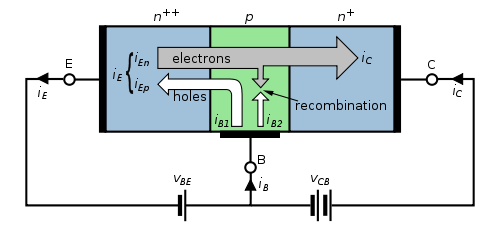
\includegraphics[width=10cm]{png/NPN_BJT_Basic_Operation_(Active)} 
\caption{\engt{An NPN transistor when the junction is active}
\nedt{Een NPN transistor als de overgang open staat.}}
\label{f:NPNactive}       % Give a unique label
\end{figure}

\engo{\begin{doE}
      We can switch on and off a LED using a NPN transistor. We should be able to reduce the current over the Base of the NPN and still obtain a functioning circuit. So, add a resistor between pin 11 and the base of the NPN. How high can you go with the resistor? Could this be a way to test the strength of the resistor?
     \end{doE}
}
\nedo{\begin{doN}
      We kunnen een LED aan en af schakelen met een NPN transisor. We zouden in staat moeten zijn om de stroom over de Basis van de NPN te verminderen en toch een werkend circuit overhouden. Probeer dit, voeg een weerstand toe tussen pin 11 en de basis van de NPN. Hoe hoog kan je gaan met de resistor? Zou dit een manier kunnen zijn om de sterkte van de resistor te testen?
     \end{doN}
}

\subsection{\engt{Analog pulse width modulation} \nedt{Analoog puls breedte moduleren}}
\eng{If you did the Task in the first section, you know that by blinking fast you can create the impression of a LED that is always on. However, as the LED was not on all the time, the LED was less bright! So, we can influence how bright a LED will be by not having it switched on all the time. The trick is to avoid seeing the LED blinking. Fortunately, humans have \href{http://en.wikipedia.org/wiki/Persistence_of_vision}{Persistence of vision}. Persistence of vision is the phenomenon where an image that is seen for only a fraction of a second will continue to be "seen" by your brain even after the original image has vanished or moved. This is the same principle behind film and television, where a rapidly changing image tricks your brain into seeing continuous motion. By turning our LED on and off rapidly, we can trick the brain into seeing an "average" value of brightness. Humans see 24 images per second, so if we switch on and off in roughly 40 milliseconds, we will not discern that the LED is blinking, but will instead see it less bright! 

We can use the \ardo{delay} function of arduino to achieve this: blinking the LED for the required amount of time. Fortunately, there is an easier way: Pulse Width Modulation (PWM). In this, a block wave is generated over a digital pin of the arduino. A block wave is a wave between 0 (off) and 1 (on). In arduino, you use the \ardo{analogWrite} function on a digital pin to achieve this. See it schematically in Fig.~\ref{f:PWM}. Note that older Arduino's only allow this on pin 9,10 and 11! So check where your version of Arduino allows this function, You recognize these pins on the board with the sign \~.

The function is called analogWrite because it is a wave over a digital pin. Analog always refers to waves, whereas digital refers to 0 and 1s. So if you make a wave with 0 and 1 (see the figure to see it is a wave), we call it again analog. The function analogWrite allows a value from 0 (=always off) to 255 (=always on). 
}

\ned{Als je de opdracht uit de eerste sectie gedaan hebt, weet je dat door vlug te blinken, je de illusie kunt cre\"eren dat de LED altijd aan is. Evenwel, de LED is niet de hele tijd aan, bijgevolg was de LED wel minder helder! Dus, we kunnen be\"{\i}nvloeden hoe helder een LED is door deze te doen blinken. De truck is te verhinderen dat de mensen hem effectief zien blinken. Gelukkig hebben mensen persistentie van beelden, denk aan de \href{http://nl.wikipedia.org/wiki/Phenakistiscoop}{Phenakistiscoop}, uitgevonden door de Belg Plateau in Gent. Persistentie van beelden is het fenomeen waarbij een beeld dat maar een fractie van een seconde gezien is, door je brein zal blijven gezien worden, zelfs nadat het originele beel verdwenen is of bewogen heeft. Dit is het principie achter film en televisie. Door de LED vlug aan en af te schakelen, kunnen we onze brein bedotten in het zien van een ``gemiddelde'' waarde van helderheid. Mensen zien 24 beelden per seconde, als we dus aan en af schakelen in ongeveer 40 milliseconden, zullen we niet in staat zijn te zien dat de LED aan het blinken is, maar zullen we in plaats daarvan een gedimd licht zien!

We kunnen de \ardo{delay} functie van arduino gebruiken om dit te programmeren: de LED aan en af zetten voor een bepaalde tijd. Gelukkig kan het eenvoudiger: Puls Breedte modulatie (PWM). In deze wordt een blokgolf gegenereerd over een digitale pin van de arduino. Een blokgolf is een golf tussen 0 (af) en 1 (aan). In arduino doe je dit met de \ardo{analogWrite} functie op een digitale pin. Zie het schematisch in Fig.~\ref{f:PWM}. Merk op dat oudere Arduino's dit enkel toelaten op pin 9,10, en 11! Controleer waar jouw versie van Arduino dit toelaat, je herkent de pins op het bord met het teken \~.

De functie wordt analogWrite genoemd omdat het een golf is over een digitale pin. Analoog refereeert altijd aan golven, terwijl digitaal refereert naar nullen en eenen. Als je dus een golf maakt met 0 en 1 (zie de figuur dat het inderdaad op een golf lijkt), noemen we het opnieuw analoog. De functie analogWrite laat waardes toe van 0 (=altijd af) tot 255 (=altijd aan).
}

\begin{figure}
  \centering
  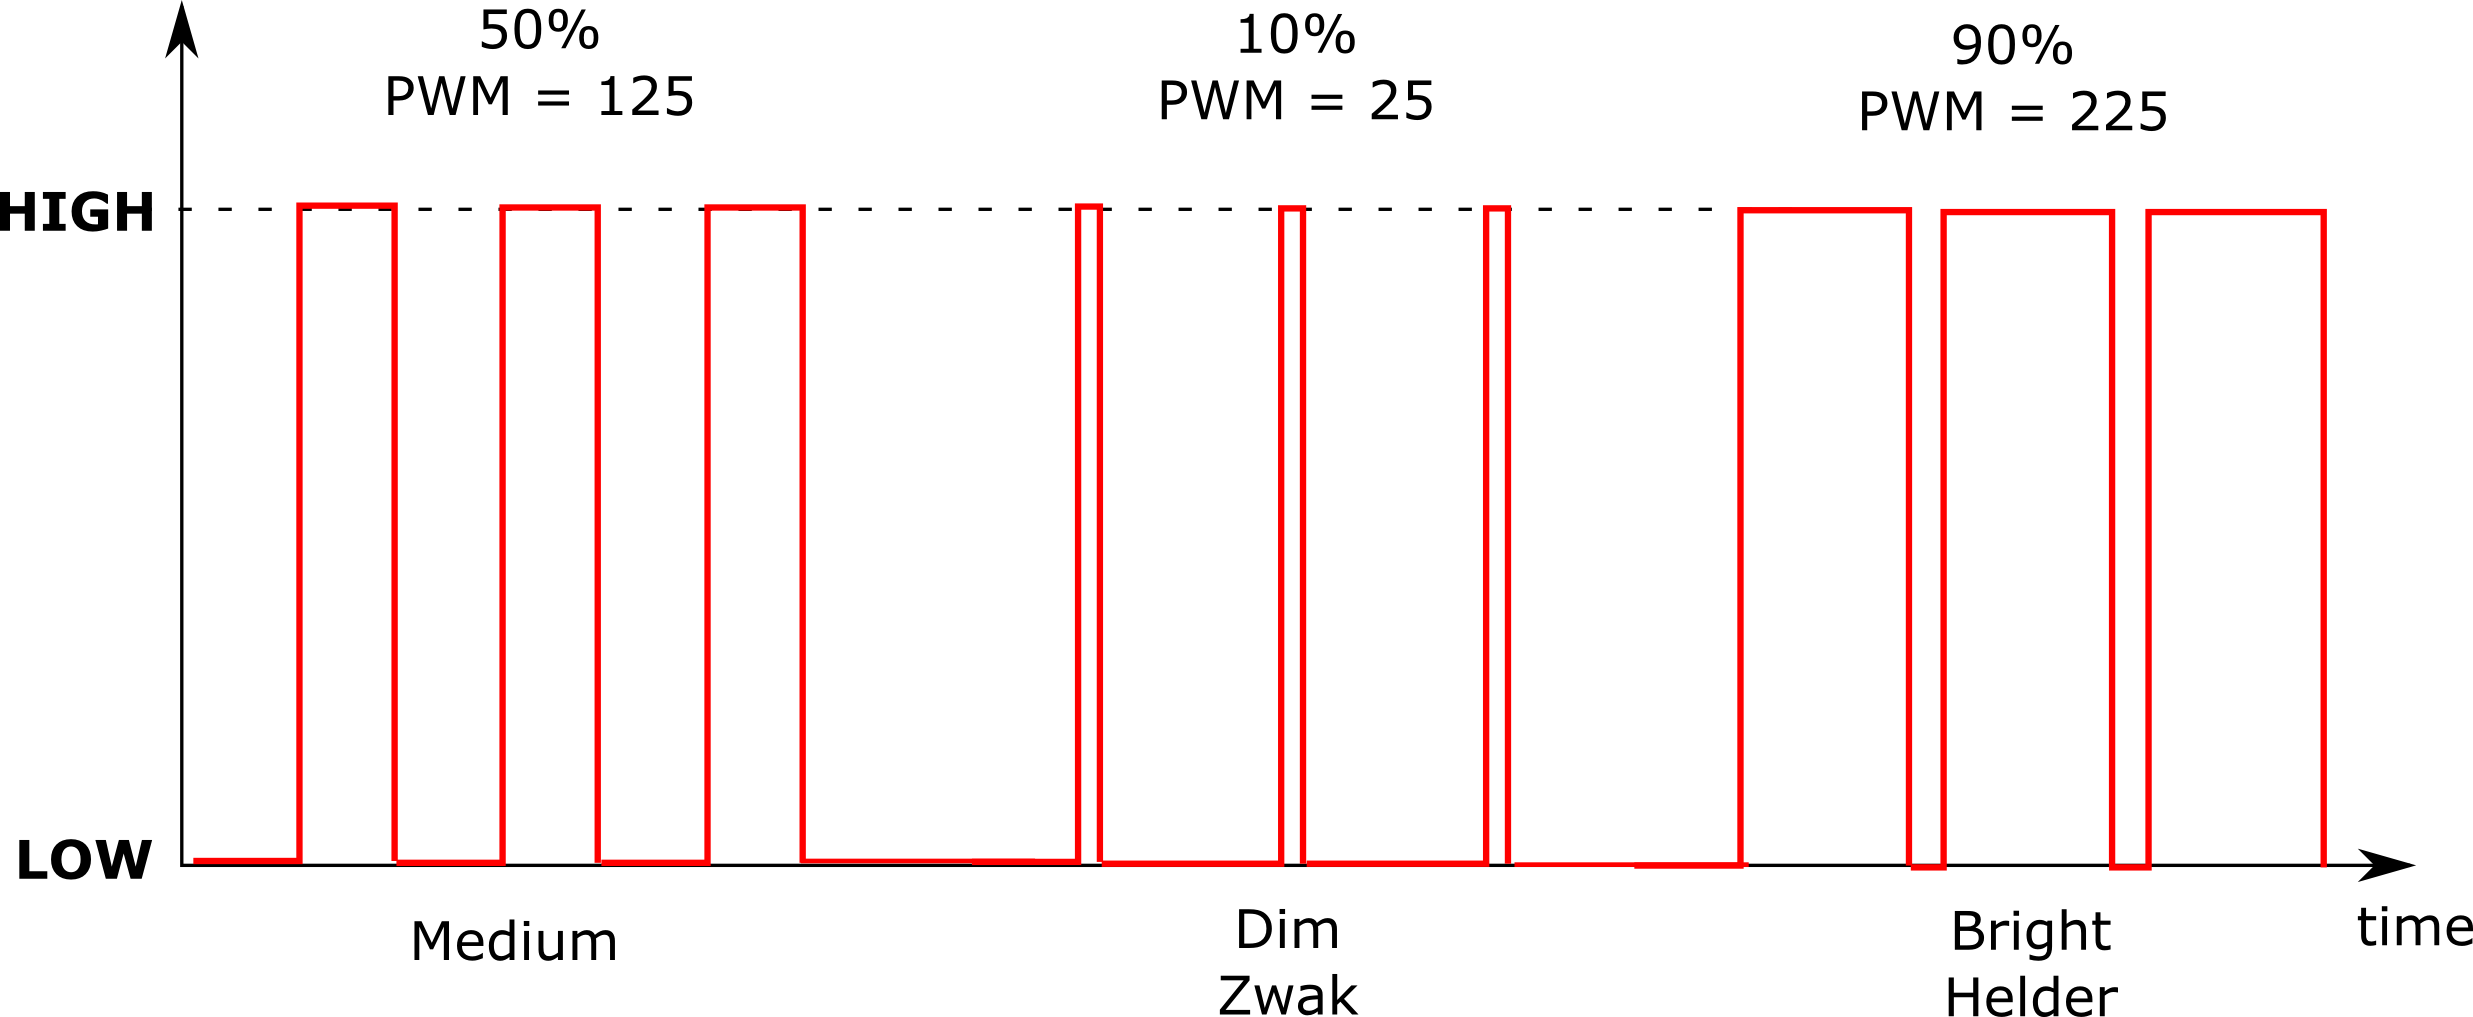
\includegraphics[width=11cm]{png/PWM} 
\caption{How PWM works in practice: over the pin a block wave is generated. - Hoe PWM in de praktijk werkt: over de pin wordt een blokgolf gegenereerd.}
\label{f:PWM}
\end{figure}

\begin{figure}
  \centering
  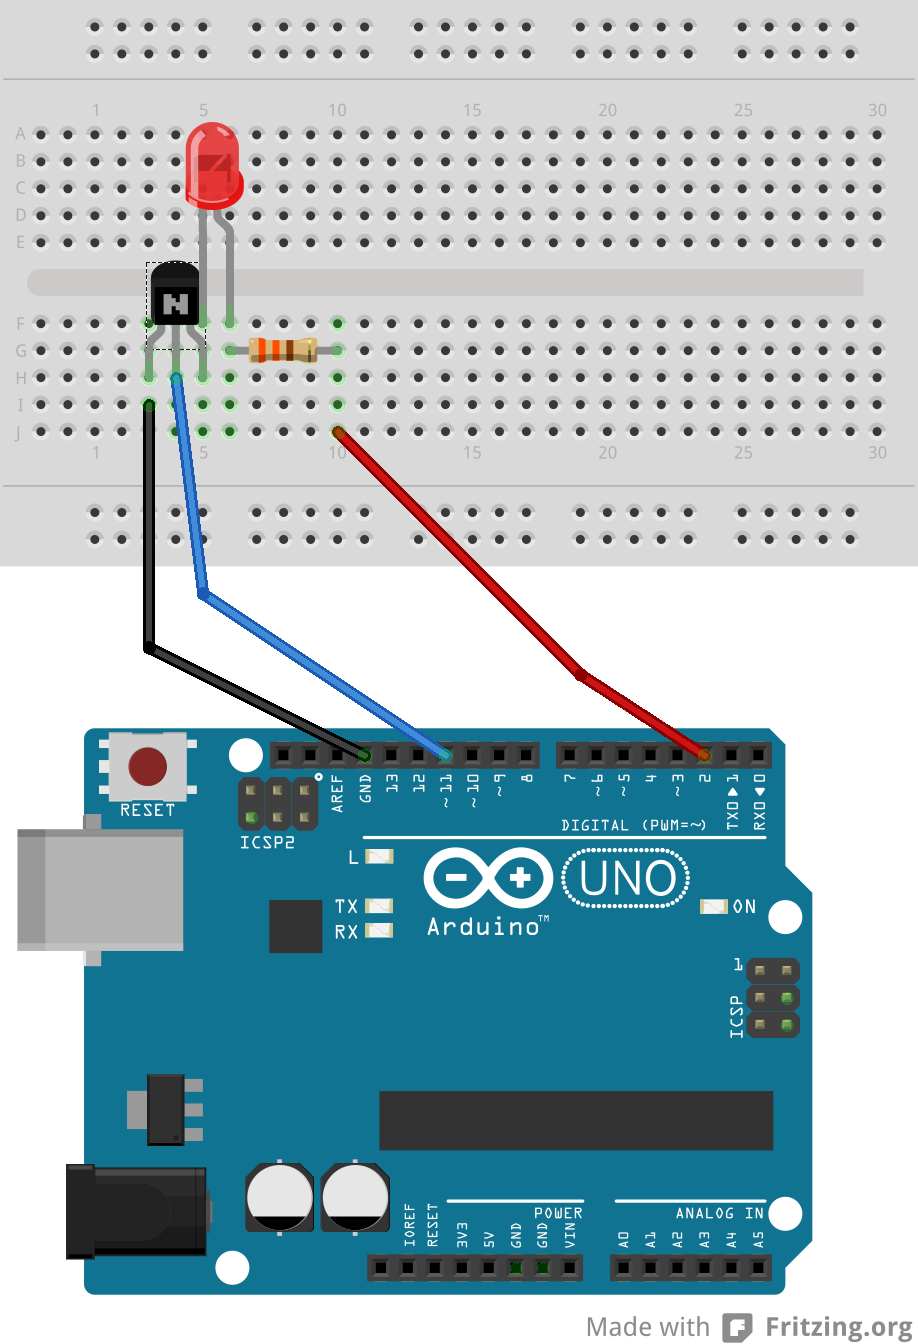
\includegraphics[width=6cm]{img/02_twopin_oneled_npn_bb} \ \ 
  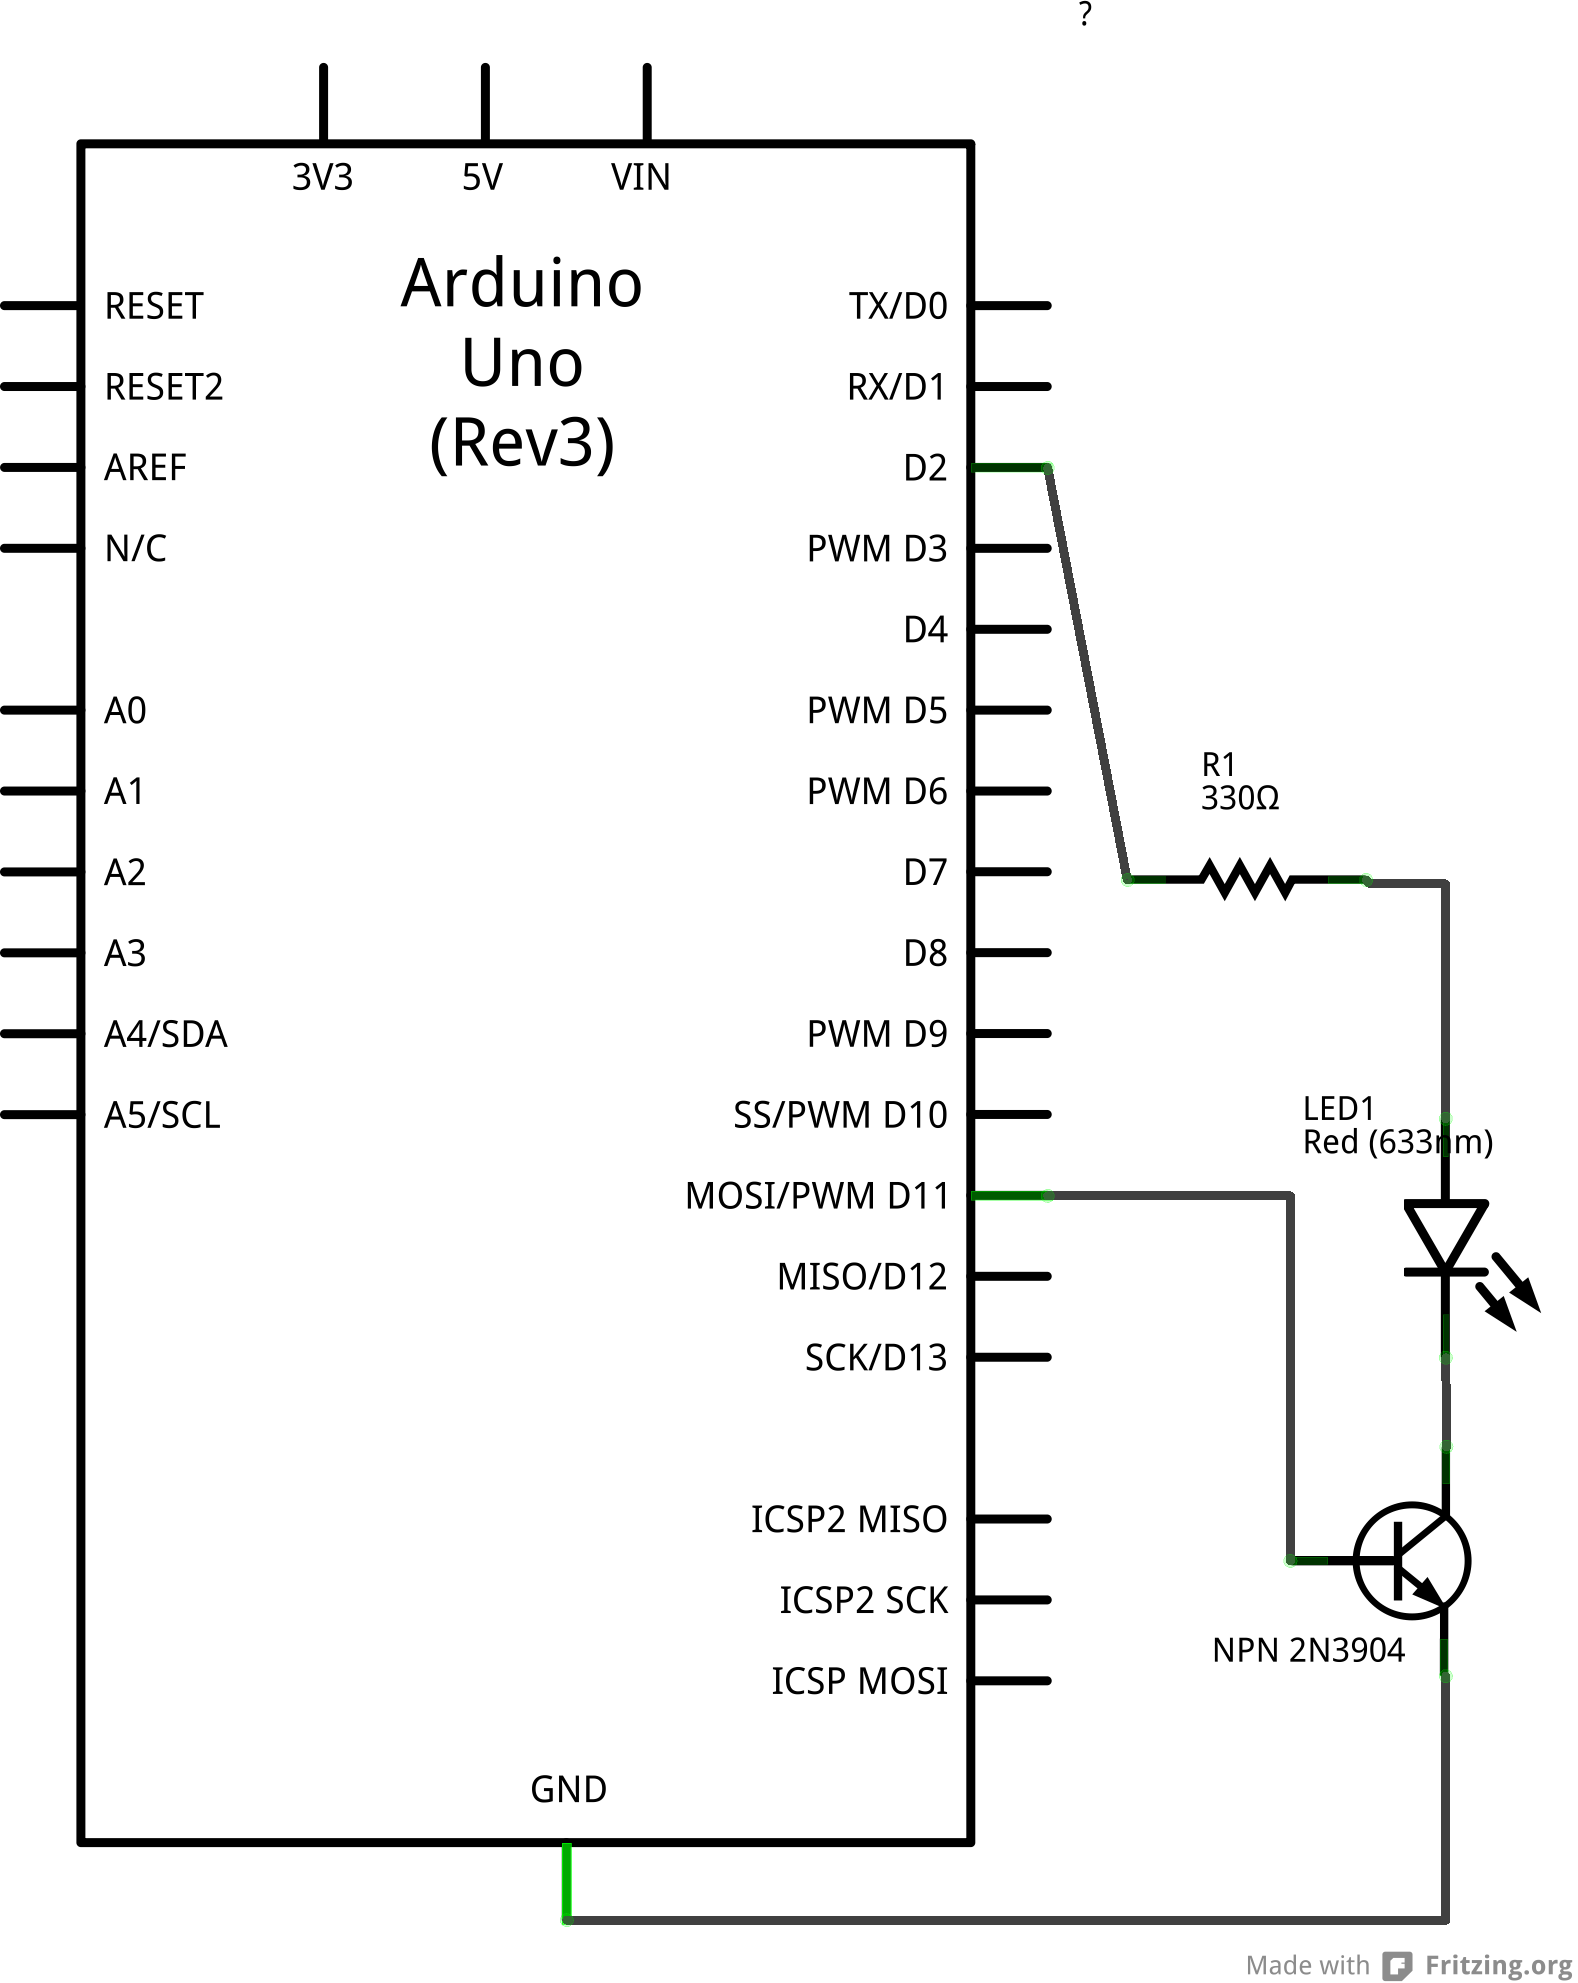
\includegraphics[width=6cm]{img/02_twopin_oneled_npn_schem}
\caption{\engt{The circuit to use PWM to change the brightness. Yes, it is identical to the previous one, all changes are in code}
\nedt{Het circuit om PWM te gebruiken om de helderheid te wijzigen. Ja, het is identiek aan het eerdere circuit, alle wijzigingen zijn in software.}}
\label{f:lesson1_twopin_PWM}       % Give a unique label
\end{figure}

\eng{The next question is then where to apply the \ardo{analogWrite}, to the NPN pin or to the led anode pin? As we learned in the previous part, it does not matter, both will interrupt the light!. We will apply it to the NPN because that is what we will use in the Fe cube. The circuit is given in Fig.~\ref{f:lesson1_twopin_PWM}. If you compare with Fig.~\ref{f:lesson1_twopin}, you see the circuit is the same. To see how to use PWM (analogWrite), see then the code below.

In this code we do one more trick. We use a random number to decide how bright the LED should be, and change this brightness every second. For this we introduce 2 new concepts:
\newline
 \textbullet\ \ardo{randomSeed(analogRead(0));} A random number is only really fully random if we cannot guess where it starts. For this we need to ``seed'' the random number generator. We do this here by reading the value on the not used analog pin 0. As analog pin is connected to nothing, there will be random noise which we cannot guess, allowing us to set our random seed to an unknown beginning. Like this we are sure the sequence of brightness we see is every time different when we switch on the Arduino.
\newline
  \textbullet\ \ardo{random} This function of arduino returns a random number; \ardo{random(256)} returns a random number between 0 and 255, see {\url{http://arduino.cc/en/Reference/random}}.
}

\ned{De volgende vraag is op welke pin we de \ardo{analogWrite} moeten toepassen. Zoals we geleerd hebben in het vorige stuk: het doet er niet toe, beide zullen de LED onderbreken. Wij zullen het toepassen op de NPN pin, gezien dat degene is die we bij de Fe cube zullen gebruiken. Het circuit is gegeven in Fig.~\ref{f:lesson1_twopin_PWM}. Als je vergelijkt met Fig.~\ref{f:lesson1_twopin}, zie je dat het circuit hetzelfde is. Zie dan om te zien hoe PWM gebruikt wordt de code hieronder.

In de code doen we nog een enkele nieuwe truck. We gebruiken een willekeurig (=random) getal om te bepalen hoe helder de LED moet zijn, en wijzigen de helderheid elke seconde. Hiertoe hebben we 2 nieuwe begrippen nodig:
\newline
 \textbullet\ \ardo{randomSeed(analogRead(0));} Een random getal is enkel volledige willekeurig indien we niet kunnen raden waar het start. Hiertoe moeten we de random getallen generator zaaien (seed in het Engels) met een begingetal. We doen dit hier door het lezen van de waarde op de niet gebruikte analoge pin 0. Gezien deze analoge pin bij ons met niets geconnecteerd is, zal er enkel willekeurige storing erop zitten, welke we niet vooraf kunnen raden. Dit zal ons ongekend begin zijn, zodat we zeker zijn dat de serie helderheid die we zien telkens anders is als we de arduino heropstarten.
\newline
 \textbullet\ \ardo{random} Deze Arduino functie genereert een willekeurig getal. Door te schrijven  \ardo{ramdom(256)} bekomen we een willekeurig getal tussen 0 en 255, zie \url{http://arduino.cc/en/Reference/random}.
\
}

\begin{code}\label{c:l1_c}
 \ \newline
\inputardfull{\string"../sketches/Fe_cube_01_led_npn_pwm/Fe_cube_01_led_npn_pwm.ino\string"}
\end{code}

\subsection{\engt{Turn it around!} \nedt{Draai het om!}}
\eng{We have used a digital pin for the plus, and the ground for the minus. In reality the pin was on 5 Volt above the ground, so we can interpret is as the ground being 0 Volt. You might think that this means pins are always positive, but that is not true. Pins can be sinks (provide negative current) or sources (provide positive current), depending on their place in the circuit. It is however important to keep in mind they can only carry a limited amount of current: 40 mA (milliamps) can be delivered to other devices/circuits. This is enough current to brightly light up a LED (don't forget the series resistor), or run many sensors, but not enough current to run most relays, solenoids, or motors. Drawing more current through a pin will destroy the pin, and possibly even the entire Arduino board! So be careful in how to use them. 

If you need more current, use the provided voltages on the board. You see a 3.3V (max 50 mA power draw) and a 5V (draw depending on how the Arduino is powered, USB or battery) pin. Test this. Make the circuit, and load the code from Code \ref{c:l1_b}. Instead of connecting the positive side to pin 1, connect it to 3.3V, and then to 5V. You will see the led works without problems, however, you no longer can interrupt the led by sending signals to pin 1.

The lesson to remember is that for big projects you should use the voltage pins on the arduino: 3.3V, 5V and GND to deliver the current, while you use the numbered pins for small things: a sensor, a led, or an NPN gate to block current. 

To experiment with the possibilities, let's completely reverse the example, and remove the ground from the circuit, using a digital pin to provide the ground. Your circuit should look like the left one in Fig~\ref{f:lesson1_twopin_PWM_reversed}. The important change is that we must set the pin 1 on 0V. This is done with a 
\ardo{digitalWrite(1, LOW);}. That is the only change in the code, but the circuit has been completely reversed

As this is a led, we use less than 40mA of current, so we can remove also the input voltage and only use pins, as in the right part of Fig~\ref{f:lesson1_twopin_PWM_reversed}.

It should be clear we can use the digital pins in different ways. Nevertheless, be well aware of the limitation to only draw 40mA from a digital pin! If you need more, use the voltage pins and the GND pin.
}

\ned{We hebben een digitale pin gebruikt voor de plus, en de grond voor de min. In realiteit was de pin op 5 Volt boven de grond, we kunnen dat dus interpreteren als de grond zijnde 0 Volt. Je zou kunnen denken dat dit betekent dat de pinnen altijd positief moeten zijn, maar dat is niet waar. Een pin kan zowel positieve stroom leveren als negatieve stroom, afhankelijk van de plaats in het circuit. Het is evenwel belangrijk om er rekening mee te houden dat een digitale pin maar een beperkte hoeveelheid stroom kan leveren: 40 mA (milliamps) is beschikbaar voor gebruik in het circuit. Dit is genoeg stroom om een LED helder te doen oplichten (vergeet evenwel geen weerstand in serie te plaatsen), of of om verschillende sensoren aan te drijven, maar niet genoeg om een relay of motor aan te drijven. Meer stroom trekken uit een digitale pin zal de pin kapot maken, en misschien wel je volledige Arduino bord! Wees dus voorzichtig in hoe je ze gebruikt.

Als je meer stroom nodig hebt, gebruik de beschikbare volt pinnen op het bord. Je ziet een 3.3V (tot 50mA stroom beschikbaar) en 5V pin (stroom afhankelijk van hoe je arduino stroom krijgt, via USB of batterij) pin. Test dit. Maak het circuit en laad de code van Code \ref{c:l1_b}. In plaats van de positieve zijde te verbinden met pin 2, connecteer ze met 3.3V en dan met 5V. Je zal zien dat de led zonder probleem werkt, maar je kan natuurlijk niet langer de led afzetten door signalen te sturen naar pin 1.

Wat je moet onthouden is dat je voor grote projecten de voltage pinnen op de arduino moet gebruiken om stroom te leveren: 3.3V, 5V en GND; terwijl je de genummerde pinnen gebruikt voor kleine dingen: een sensor, een led, of een NPN transistor om stroom te onderbreken.

Om te experimenteren met de mogelijkheden, laat ons het vorige voorbeeld helemaal omdraaien, en de grond verwijderen uit het circuit door een digitale pin te gebruiken als grond. Jou circuit zou eruit moeten zien als de linkse uit Fig~\ref{f:lesson1_twopin_PWM_reversed}. Belangrijk hier is dat we pin 2 moeten plaatsen op 0V. Dit doen we met
\ardo{digitalWrite(1, LOW);}.  Dat is de enige wijziging bij de vorige code, maar het circuit is wel omgedraaid!

Gezien dit een led is gebruiken we minder dan 40mA stroom, en kunnen we dus ook het input voltage vervangen door een pin, zoals gedaan in de rechterfiguur van Fig~\ref{f:lesson1_twopin_PWM_reversed}.

Het zou duidelijk moeten zijn dat we de digitale pinnen op verschillende manieren kunnen gebruiken. Wees je evenwel goed bewust van de limitatie van de pinnen: je kan enkel 40mA uit een digitale pin krijgen. Als je meer nodig hebt, gebruik de voltage pinnen en de GND pin.
}

\begin{figure}
  \centering
 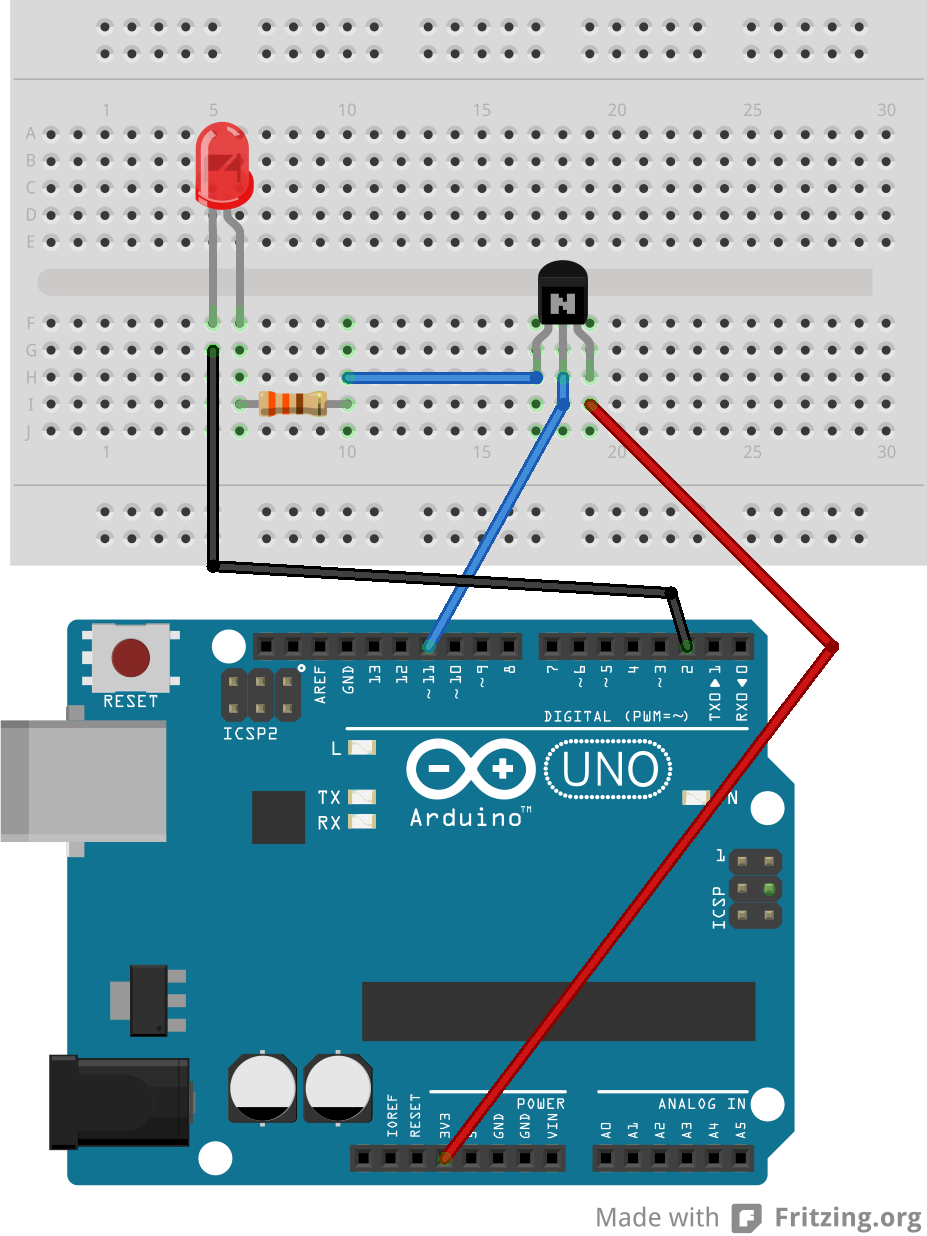
\includegraphics[width=5cm]{img/03_twopin_oneled_npnreversed_bb} 
 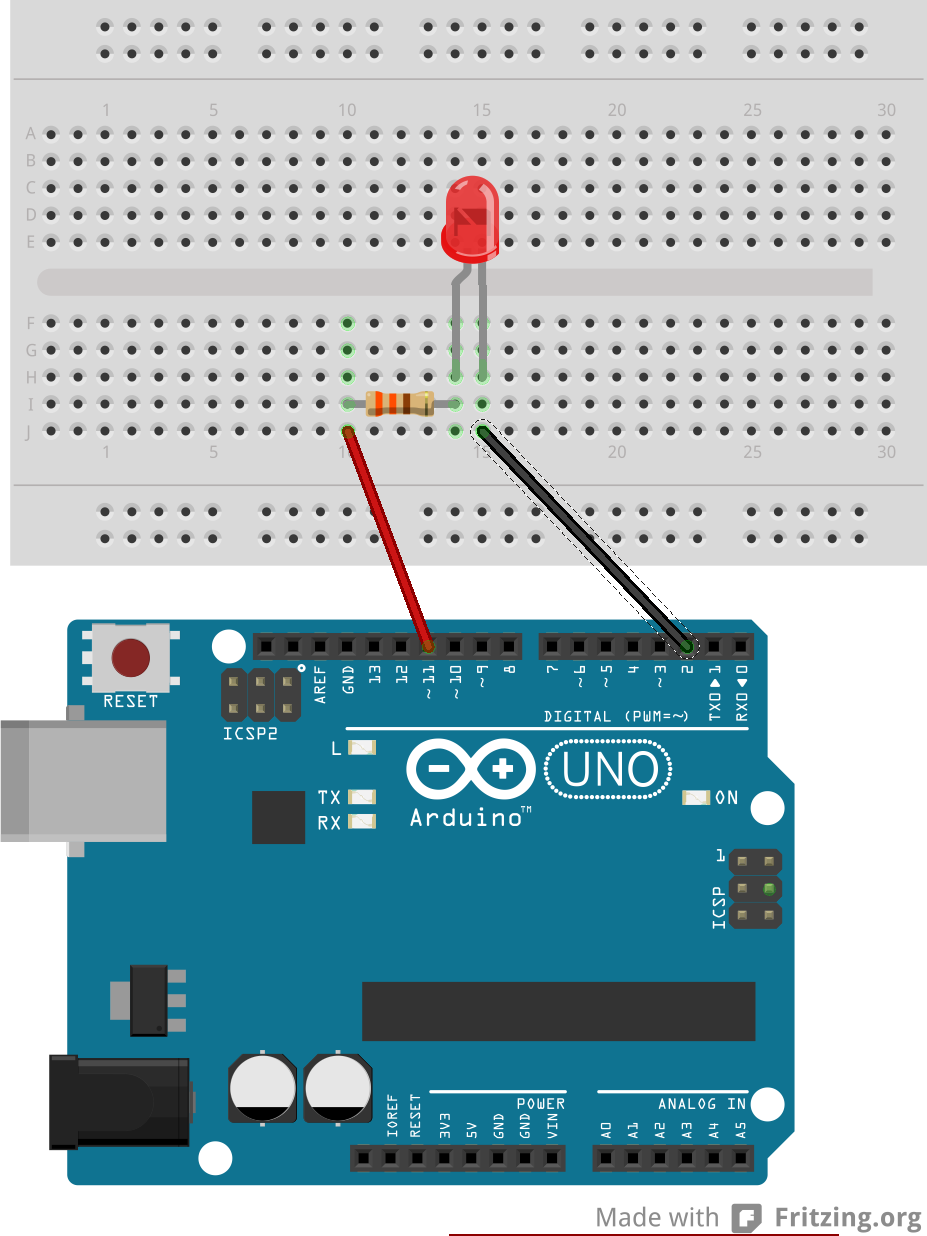
\includegraphics[width=5cm]{img/03_twopin_oneled_npnreversed2_bb} 
\caption{\engt{Using two pins and an NPN gate, we can switch off the LED on both sides. Now we use pin 2 to allow a sink at the pin. Right: Removing the NPN makes for a simpler circuit}
\nedt{Met twee pinnen en een NPN brug kunnen we de LED afzetten aan beide kanten. We gebruiken nu pin 2 zodat we de pin als grond kunnen gebruiken. Rechts: De NPN verwijderen zorgt voor een eenvoudiger circuit.}}
\label{f:lesson1_twopin_PWM_reversed}
\end{figure}

\eng{Note following thing in the code: As pin 2 needs to act as ground, we need to do \ardo{digitalWrite(LOW)} on this pin. }
\ned{Merk het volgende op in de code: gezien pin 2 zich als grond moet gedragen dienen we \ardo{digitalWrite(LOW)} op de pin uitvoeren.}

\begin{code}\label{c:l1_d}
 \ \newline
\inputardfull{\string"../sketches/Fe_cube_01_led_npn_pwm_reverse/Fe_cube_01_led_npn_pwm_reverse.ino\string"}
\end{code}


\section{\engt{Lesson 2: A RGB Led Circuit} \nedt{Les 2: Een RGB Led circuit}}

\subsection{\engt{The RGB circuit} \nedt{Het RGB circuit}}
\begin{figure}[ht]
  \centering
  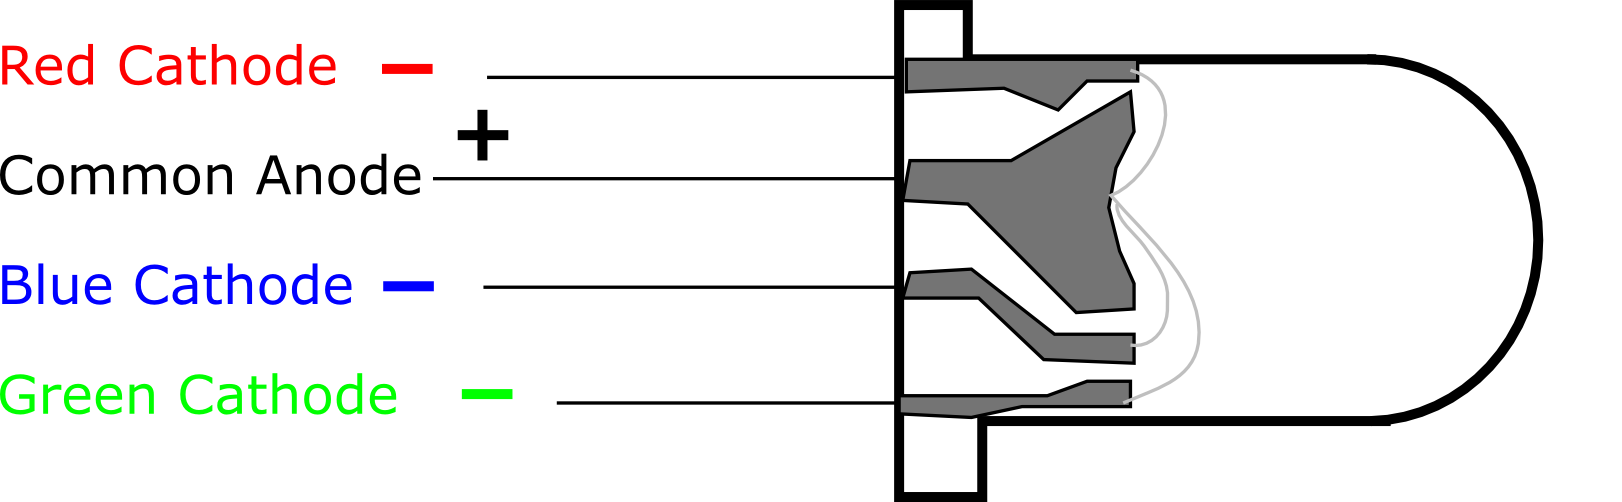
\includegraphics[width=6cm]{png/RGB_LED2}
  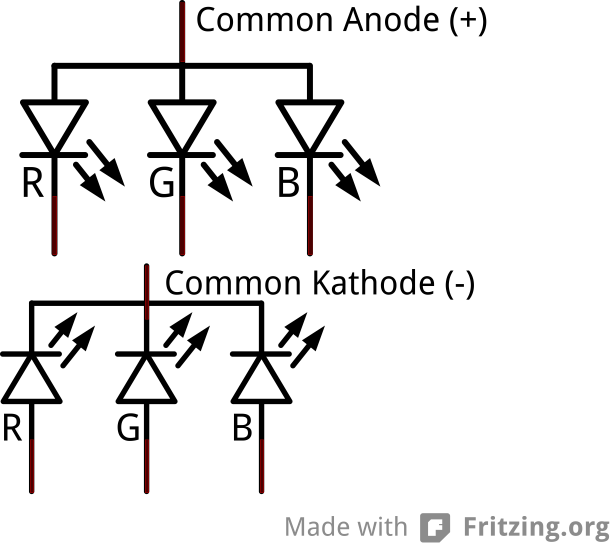
\includegraphics[width=3cm]{png/RGB_Led_schem} 
\caption{\engt{Left a blow up of an RGB Led with common anode, Right a schematic version used in circuits} \nedt{Links een vergroting van een RGB led met gedeelde anode, Rechts een schema zoals je in circuits kan vinden.}}
\label{f:RGB_LED}
\end{figure}

\eng{Led exist in different colors. Some leds can produce a color range. These are RGB leds, see a depiction in Fig.~\ref{f:RGB_LED}. They are essentially a red, green and blue led rolled in a single package, and with a common anode or a common kathode. To drive this led, we extend the single led circuit with NPN. We assume you have an RGB led with 3 cathodes and one anode, so we need 3 NPN gates, but only one resistor. 

\textbf{Note:} If you use a led with a common kathode, you will need to turn the circuit around as given in the previous lesson. See the cube later on where this is the case.
}

\ned{Led bestaan in verschillende kleuren. Sommige led kunnen een kleurenbereik produceren. Dit zijn RGB leds, zie een afbeelding in Fig.~\ref{f:RGB_LED}. Ze zijn in essentie een rode, groene en blauwe led in een enkel pakket, met een gedeelde anode of een gedeelde kathode. Om deze led aan te drijven breiden we ons 1 led met NPN circuit uit. We veronderstellen dat je een RGB led hebt met 3 kathoden en 1 anode, dus zullen we 3 NPN bruggen nodig hebben, en 1 resistor. 

\textbf{Merk Op:} Indien je een led gebruikt met een gedeelde kathode dien je het circuit om te draaien zoals gezien in de vorige les. Zie ook de kubus later waar dit het geval is.
}


\engo{\begin{doE}
      \textbf{Test your RGB LED}. So, there are 4 legs to the RGB LED. The longest one is or the common kathode (-, connect to GND) or the common anode (+, connect to a voltage). You will need to test your LED to know which is the case, and you will need to test what leg is which color. Do this now: put the RGB led on your breadboard, connect a 330$\Omega$ resistor from the row with the longest leg to another row on the breadboard. Now take two wires, and plug one in the GND, and the other in the 3.3V output. Your arduino should be powered, so connect it via usb to your PC. Assume first it is a common kathode LED, so connect the GND to the resistor. With the 3.3V wire, test the legs of the LED. Not working? Remove the wires from the breadboard and test if it is a common anode LED. So connect 3.3V wire now to the resitor, and test the other legs with the GND wire.
      
      Tip: Make a scetch of your LED, writing down what is Red, Green, Blue and the kathode/anode!
     \end{doE}
}
\nedo{\begin{doN}
      \textbf{Test je RGB LED}. Er zijn dus 4 beentjes aan de RGB LED. Het langste been is normaal de gemeenschappelijke kathode (-, verbindt met GND) of de gemeenschappelijke anode (+, verbindt met een voltage). Je zal je LED moeten testen om te weten wat wat is. Doe dit nu: plaats de RGB LED op je breadboard, connecteer een 330$\Omega$ weerstand van de rij met het langste been naar een andere vrije rij op je bord. Neem nu twee draden, en plaats een in de GND, en de andere in de 3.3V output. Je Arduino zet je aan, verbindt dus de usb kabel met je PC. Onderstel eerst dat het een gemeenschappelijke kathode LED is, dus verbindt de GND draad met de weerstand. Met de 3.3V draad test je de beentjes van de LED. Het werkt niet? Verwijder de draden van het schakelbord en test of het een gemeenschappelijke anode LED is. Dus, verbindt de 3.3V draad met de weerstand, en test de andere LED beentjes met de GND draad.
      
      Tip: Maak een schets op papier van je LED, waarbij je noteert welk been Rood, Groen en Blauw is, alsook de kathode/anode.
     \end{doN}
}


\begin{figure}
  \centering
  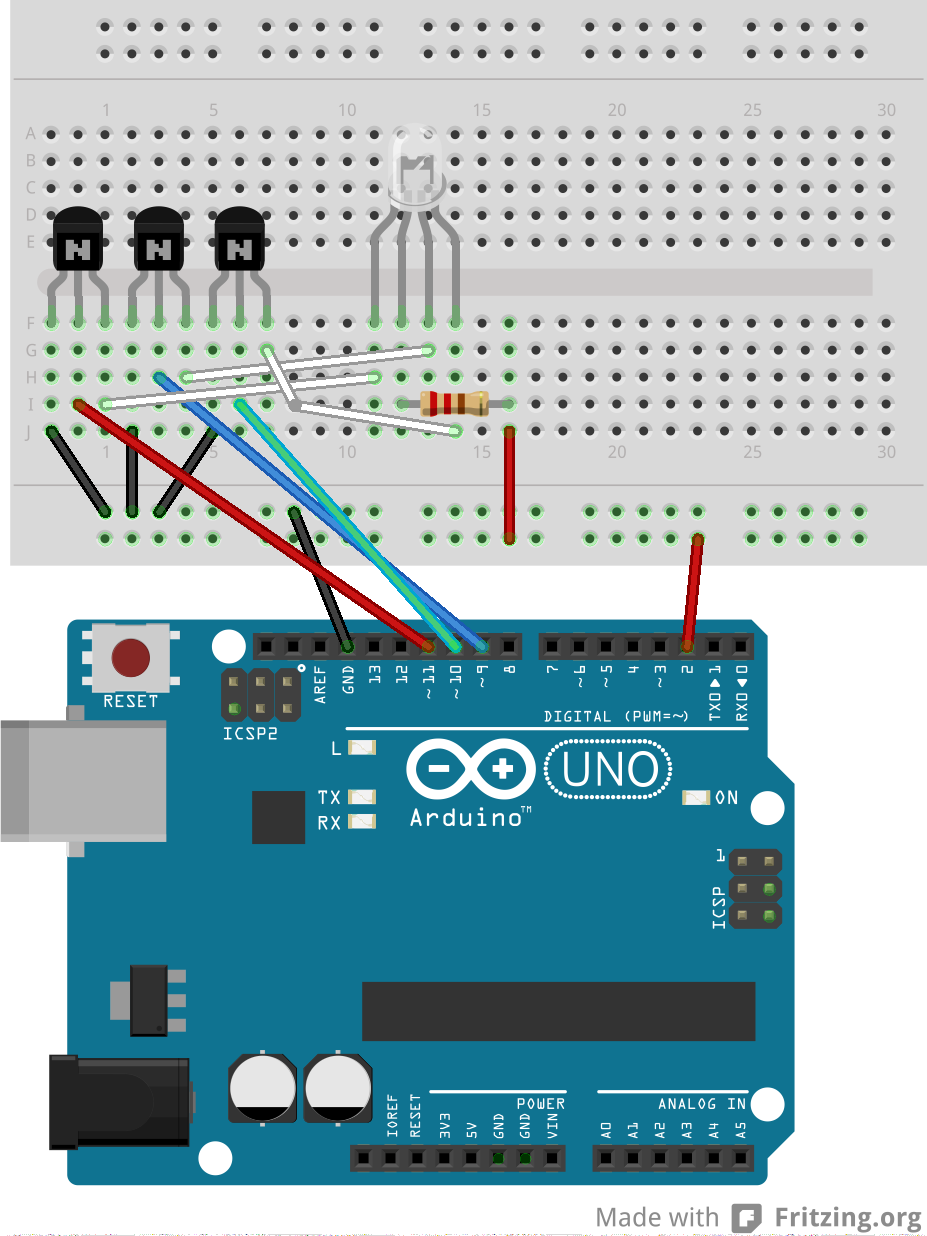
\includegraphics[width=6cm]{img/04_rgbled_bb} \ \ 
  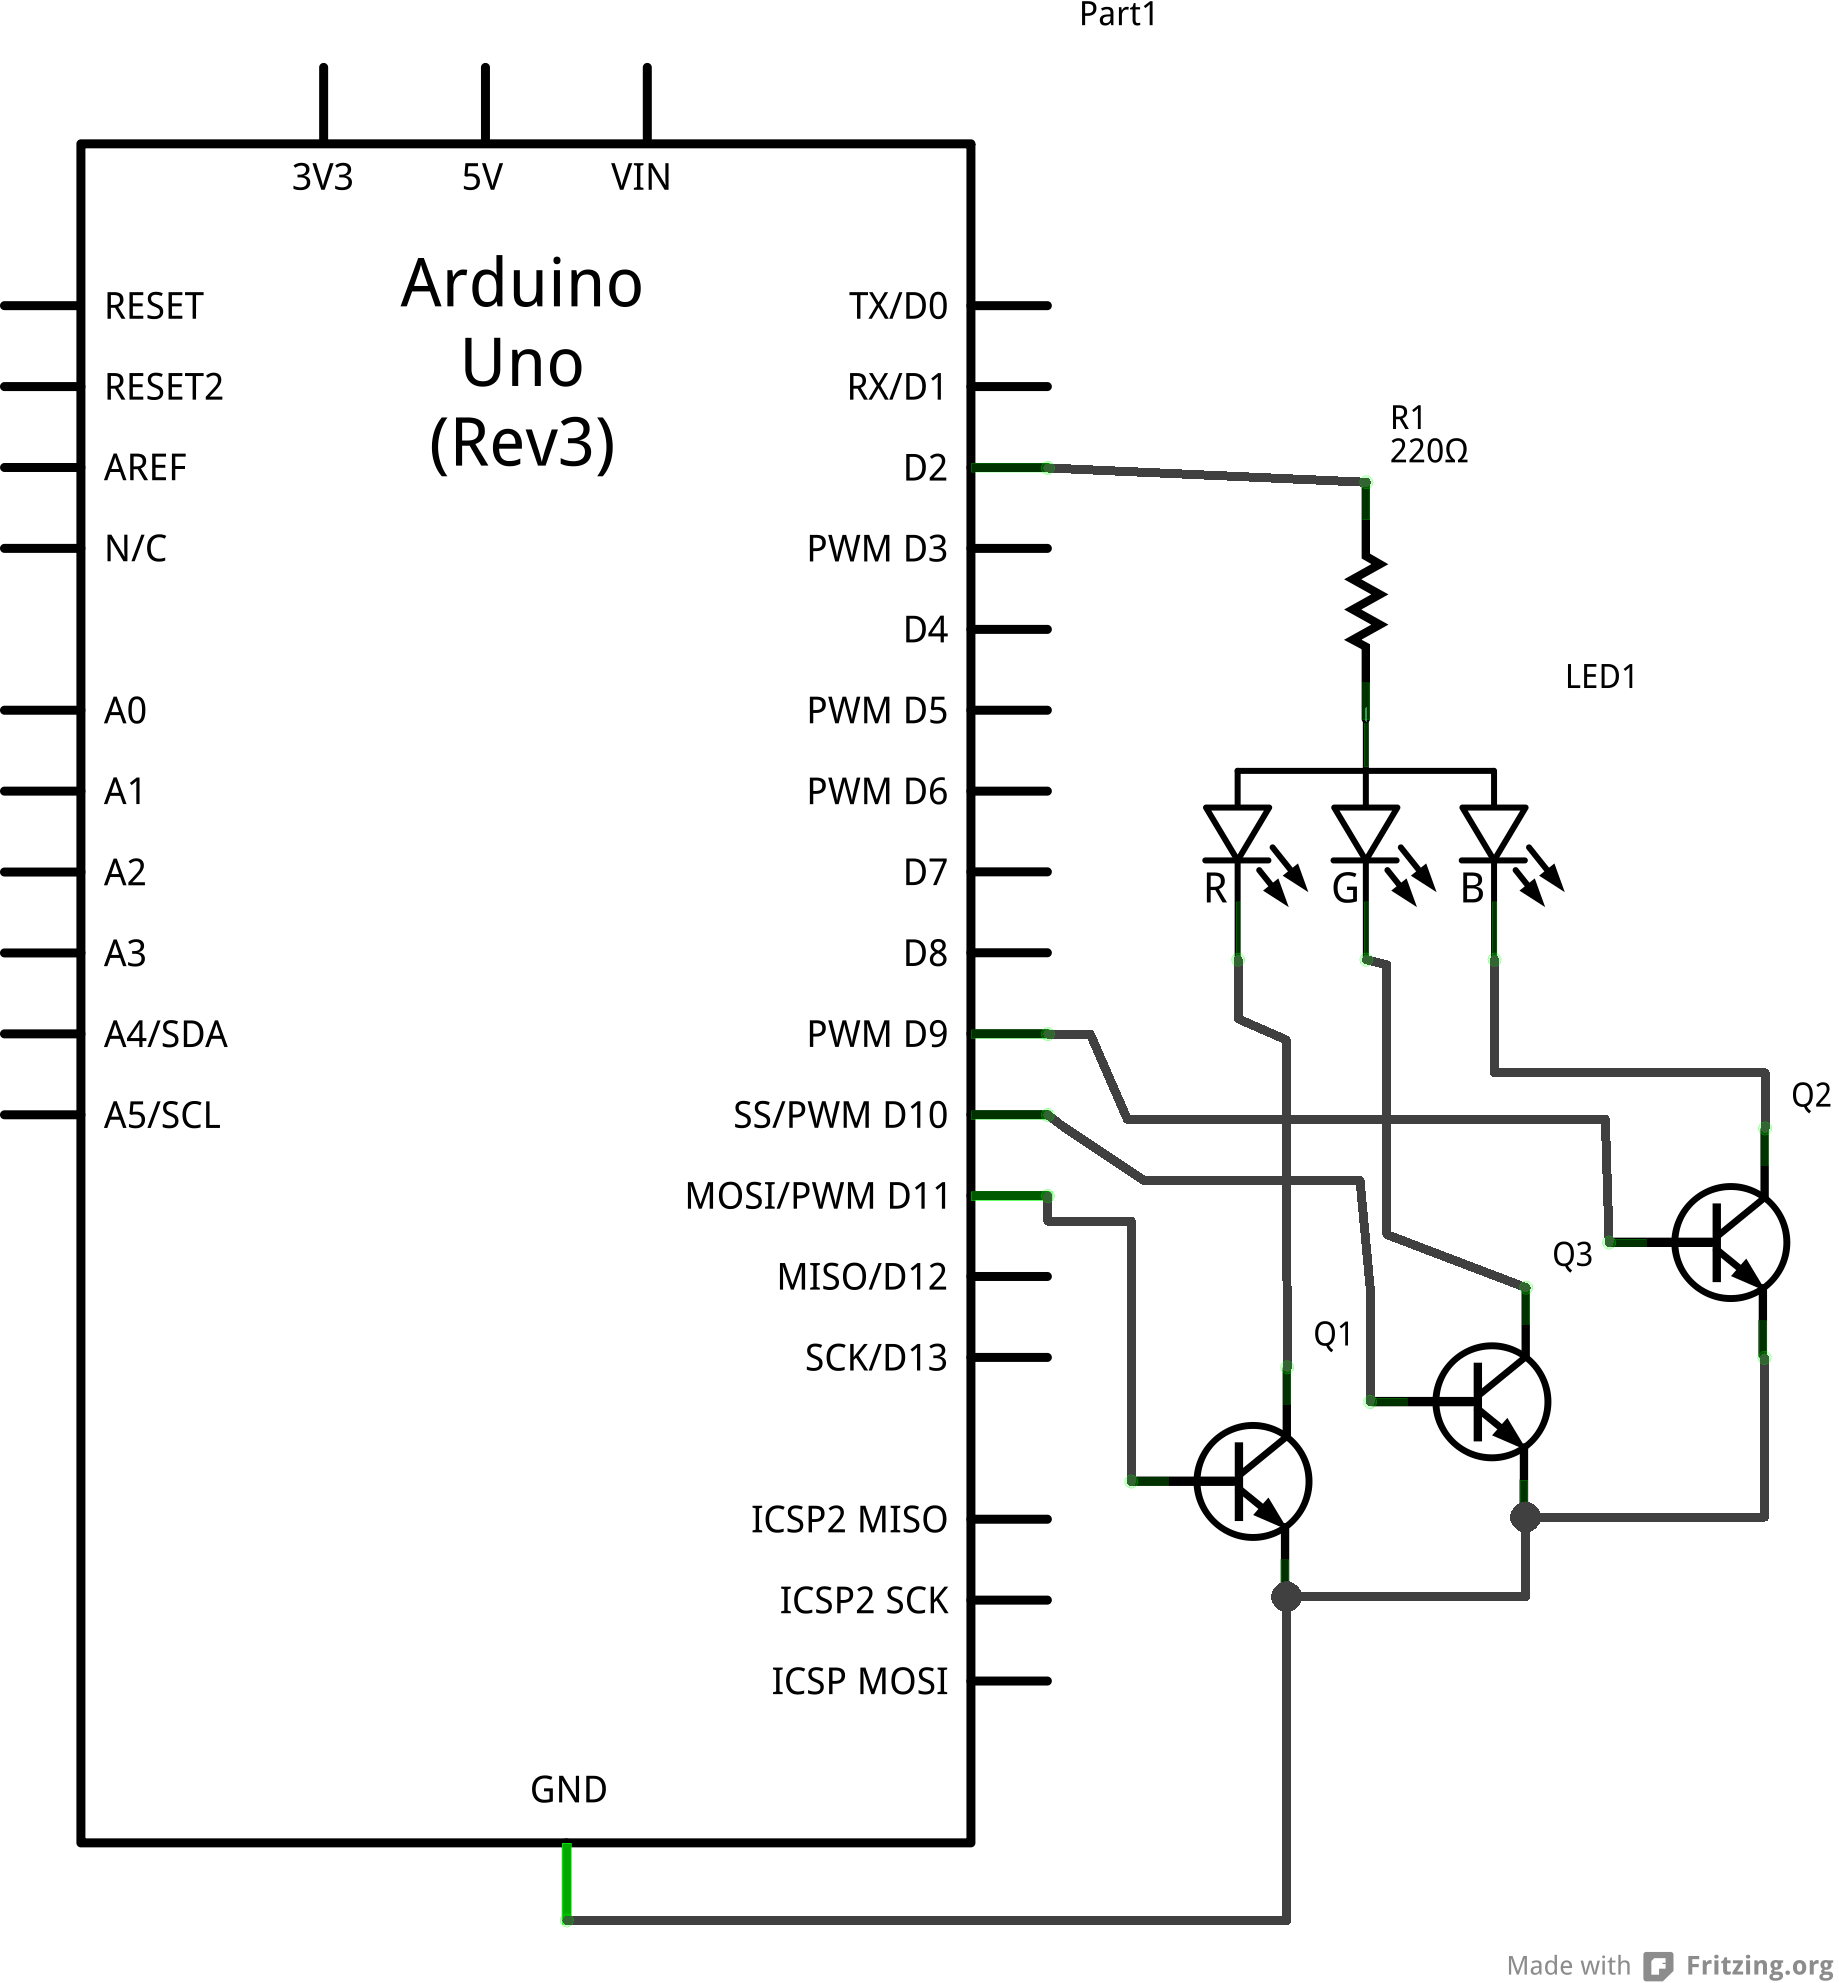
\includegraphics[width=6cm]{img/04_rgbled_schem}
\caption{\engt{Circuit for a common anode RGB Led} \nedt{Circuit voor een gedeelde anode RGB Led.}}
\label{f:lesson2_RGB}
\end{figure}

\eng{The circuit is given in Fig.~\ref{f:lesson2_RGB}. Some things to note: the NPN out (E) all connect to the ground, so connect them to a single row on your breadboard. For the other connections, different wires are needed: 4 control pins and the ground, so 5 wires. 

Once you have the circuit made, the rest of the lesson will be programming the led. Start with a simple program to have the Led cycle through Red, Green and Blue. When finished, make sure this is indeed the order, if not, you made an error wiring the Cathodes. If you power two kathodes at the same time, you will obtain sometimes a nice mixed color, and sometimes not. This is because the resistance for one color is not equal to another, so the current can have a preferential path. So, cheap RGB led are not good to intermix colors by powering two or more cathodes at the same time. We will need to use tricks to nicely mix colors. That is for the next section, for this section our first arduino sketch was:}

\ned{Het circuit is gegeven in Fig.~\ref{f:lesson2_RGB}. Enkele dingen om rekening mee te houden: De NPN uit (E) gaan allemaal naar de grond (GND), plaats ze dus op een enkele rij op je schakelbord. Voor de andere connecties heb je verschillende draden nodig: 4 controle pinnen en de grond, dus 5 draden.

Eenmaal je het circuit gemaakt is, is het vervolg van deze les het programmeren van de led. Start met een simpel programma om de led te laten lopen door Rood, Groen en Blauw. Als je klaar bent, verifieer dat je inderdaad deze orde ziet, indien niet heb je een fout gemaakt met het bedraden van de kathoden. Als je twee kathoden terzelfdertijd onder stroom plaats, zul je soms een mooie gemengde kleur krijgen, en soms niet. Dit is omdat de weerstand via een kleur niet identiek is aan die van een andere kleur, waardoor de stroom via een preferentieel pad zal lopen. Goedkope RGB led zijn niet zo goed om kleuren correct te mengen door twee of meer kathoden terzelfdertijd aan te sturen. We zullen enkele trukjes moeten gebruiken om kleuren mooi te mengen. Dat is voor de volgende sectie, voor deze sectie was onze eerste arduino sketch:}

\begin{code}\label{c:l2_a}
 \ \newline
\inputardfull{\string"../sketches/Fe_cube_02_RGB_npn/Fe_cube_02_RGB_npn.ino\string"}
\end{code}


\subsection{\engt{Mixing colors} \nedt{Kleuren mengen}}
\eng{In Code \ref{c:l1_c} we have shown how a led light can be dimmed. We use this now to mix colors. If we succeed in showing first red, then green, and then blue, with the colors correctly dimmed, we can mix colors. For example, if we turn off green, we will obtain red+green=yellow. The trick will again be do this all so fast that due to persistence of vision we trick the eye into seeing a non-blinking mixed color.

So, create an arduino sketch to show a random mixed color for a second, then switch to a next random color. To dim a color we use \ardo{analogWrite}. We have seen that \ardo{analogWrite} creates a block wave, and that we can create 256 different block waves. The number 256 is not arbitrary. We have that 256=2*2*2*2*2*2*2*2, so 2 is multipled 8 times with itself. This is the largest number you can create with a single byte in the Arduino memory. The so called 8 bit byte is the unit used in the first computers to store information. 

It is most fortunate that 256 is used in analogWrite, as the original computer \href{http://en.wikipedia.org/wiki/RGB_color_model\#Numeric_representations}{RGB color model} is based on this number. The colors we will make with our multicolor led should hence corresponds to those of the RGB color model, see Fig.~\ref{f:RGB_color}. 
}

\ned{In Code \ref{c:l1_c} hebben we getoond hoe we een LED licht kunnen dimmen. We gebruiken dit nu om kleuren te mengen. Als we erin slagen om eerst rood, dan groen, en dan blauw te tonen, met de kleuren correct gedimd, dan kunnen we kleuren mengen. Bevoorbeeld, als we groen afzetten zullen we rood+groen=geel krijgen. De truck om dit te doen werken zal weer zijn dat we dit allemaal zo snel moeten doen dat door persistentie van visie we ons ook kunnen doen geloven dat we op een niet pinkende manier kleuren mengen

Maak dus een arduino sketch om een willekeurige gemengde kleur te tonen voor een enkele seconde, om daarna een andere willekeurige kleur te tonen. Om een kleur te dimmen gebruiken we weer \ardo{analogWrite}. We hebben gezien dat \ardo{analogWrite} een blokgolf maakt en dat we 256 verschillende blokgolven kunnen verkrijgen, van 0 tot 255. Het nummer 256 komt niet zomaar uit de lucht vallen. We hebben dat 256==2*2*2*2*2*2*2*2, het is dus 2 die 8 keer met zichzelf vermenigvuldigd wordt. Dat is het grootste nummer die je kunt maken met een enkele byte (=8 bits) van het Arduino geheugen. De zo genaamde 8 bit byte is de eenheid gebruikt in de alereerste computers om informatie mee op te slaan.

Het is erg handig dat 256 gebruikt wordt in \ardo{analogWrite}, gezien het originele \href{http://en.wikipedia.org/wiki/RGB_color_model\#Numeric_representations}{RGB kleurenmodel} gebasseerd is op dit getal. De kleuren die wij zullen maken met onze RGB LED zullen dus overeenkomen met die van het RGB kleurenmodel, zie Fig.~\ref{f:RGB_color}. 
}


\begin{figure}
  \centering
  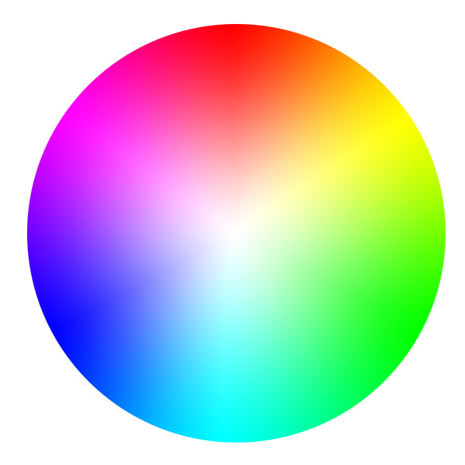
\includegraphics[width=6cm]{img/colorwheel-rgb.jpg}
\caption{Part of the RGB colors possible - Een deel van de mogelijke kleuren met RGB leds}
\label{f:RGB_color}
\end{figure}


\eng{The actual code is given in Code \ref{c:l2_b}. Several new concepts are presents.
\newline 
\textbullet\ \ardo{Serial.begin} and debugging: \ardo{Serial} allows to inspect your Arduino from your PC. It opens a slow connection to which you can print. We do this with a flag: \ardo{bool test} is a variable we call a flag: it can have two values: true or false. If the variable is true, we print on the serial connection the values of the randomly determined Red, Green and Blue value.  We do this with the command \ardo{Serial.print}. To make sure the next value of RGB is printed on a new line, we finish with \ardo{Serial.println}
\newline
\textbullet\ \ardo{millis()}: this is a function that returns the number of milliseconds since the arduino was switched on. You can find functions in the \href{http://arduino.cc/en/Reference/millis}{Reference guide}. The maximum amount will correspond to 50 days. After that it restarts from 0.
\newline
\textbullet\ An \ardo{if} test. This is a condition, if the part after the \ardo{if} in normal brackets is true, we will execute the part following in curly brackets, otherwise not. The syntax is:\newline
 \ardo{if (condition)\{ ... commands ...\}}
\newline
so 'commands' are only executed if the condition is true.
\newline 
\textbullet\ A \ardo{while} loop: This is a repetition based on a condition. As long as the condition in normal brackets is true the piece following in curly brackets will be executed. The syntax is:\newline
 \ardo{while (condition)\{ ... commands ...\}}
\newline
so 'commands' will be executed as long as condition is true. Careful here, it's easy to create while loops that never end. It's important that the condition is something that is updated regularly. In our code, the condition is:\newline
\ardo{currentTime - prevTime < 1000} \newline
so as soon as this is 1000 milliseconds the loop will stop. This will happen because in the curly brackets with the commands you see as last command:\newline
\ardo{currentTime = millis();}
\newline
so the variable currentTime is ever increasing, and the while loop will indeed stop. 
}


\ned{De gebruikte code vind je in Code \ref{c:l2_b}. Verschillende nieuwe concepten zijn aanwezig.
\newline 
\textbullet\ \ardo{Serial.begin} and \ardo{print}: \ardo{Serial} laat toe om je Arduino te observeren vanuit je PC. Het opent een trage connectie naar waar je prints kunt sturen. In de sketch doen we dat via een vlag: \ardo{bool test} is een variabele die we een vlag noemen: het kan twee waarden hebben: waar of vals, welke in het Engels zijn \textit{true} of \textit{false}. Als de variabele true is, dan printen we op de seri\"ele connectie de waarden van de willekeurig bepaalde Rood, Groen, en Blauw. We doen dit met het commando \ardo{Serial.print}. Om ervoor te zorgen dat de volgende waarde van RGB op een nieuwe lijn komt, eindigen we met \ardo{Serial.println}, die laaste \textit{ln} staat voor 'lijn'
\newline
\textbullet\ \ardo{millis()}: Dit is een fuctie die het aantal milliseconden sinds de opstart van de Arduino teruggeeft. Je kan functies opzoeken in de \href{http://arduino.cc/en/Reference/millis}{Reference guide}. Het maximum getal die je kunt terugkrijgen komt overeen met 50 dagen. Daarna herstart het van 0.
\newline
\textbullet\ Een \ardo{if} test. Dit is een conditie. Als het stuk achter de \ardo{if} in normale haakjes waar (true) is, dan wordt het stuk in gekrulde haakjes uitgevoerd, anders niet. De syntax is:\newline
 \ardo{if (conditie)\{ ... commando's ...\}}
\newline
dus 'commando's' worden enkel uitgevoerd als conditie waar is.
\newline 
\textbullet\ Een \ardo{while} lus: Dit is een repetitie gebaseerd op een conditie. Zolang de conditie waar is zal het stuk in de gekrulde haakjes uitgevoerd worden. De syntax is:\newline
 \ardo{while (conditie)\{ ... commando's ...\}}
\newline
dus 'commando's' zullen uitgevoerd worden zolang conditie waar is. Opgelet hier, het is gemakkelijk om een while loop te maken die nooit stopt Het is belangrijk dat de conditie iets is dat regelmatig aangepast wordt. In onze code is de conditie:\newline
\ardo{currentTime - prevTime < 1000} \newline
dus zolang de huidige tijd (\textit{currentTime}) min the vorige tijd (\textit{prevTime}) minder dan een seconde is, herhalen we de commando's. Er zal een moment komen waarop de conditie vals is en de lus stopt. Dit omdat je als laatste lijn in de gekrulde haken van de while ziet:\newline
\ardo{currentTime = millis();}
\newline
dus de variabele currentTime neemt constant toe, en de while loop zal inderdaad stoppen. 
}

\begin{code}\label{c:l2_b}
 \ \newline
\inputardfull{\string"../sketches/Fe_cube_02_RGB_npn_random_color_PWM/Fe_cube_02_RGB_npn_random_color_PWM.ino\string"}
\end{code}

\eng{
The Led should burn nicely, switching colors every second. However, if you play around with the \ardo{delayDuration} variable, you should quickly see that for several values the led starts to flikker, which is highly annoying.

So, to test the colors are a little bit accurate, do the following:
\begin{enumerate}
 \item change the time of a single color to 60 seconds, so 60000 milliseconds
 \item verify you have in the sketch: \ardo{bool test=true;}
 \item upload the sketch, a color will now last one minute
 \item Open the serial monitor, this is the icon with the lens in the top
right of the Arduino Editor. Every minute you will see the color values that are shown on the LED.
 \item To see if this is somewhat correct, use a color picker tool. For example \href{http://www.colorpicker.com/}{www.colorpicker.com} has fields for R, G and B to see what color corresponds with those values.
 \item Don't expect too much accuracy in these colors! First, if you don't use a dark room, the LED will always have color, so blacks are not possible. If you do use a black room, the red, green and blue are generated in different regions of the LED, so when they all burn, the mixing is not perfect. Next, the pure red, green and blue doe not exactly match those of the RGB color model, so mixing is different. Lastly, the LED produces little light, the LED actually contains or lens to focus the light in only one direction, or a dimmed packaging to diffuse the light in all directions. In both cases this creates artifacts.
\end{enumerate}
}

\ned{De LED zou moeten mooi branden, en van kleur wisselen elke seconde. Als je speelt met de variabele \ardo{delayDuration}, zul je evenwel opmerken dat de LED gemakkelijk begint te flikkeren als je niet vlug kleur wisselt.

Om te testen hoe accuraat de kleuren zijn, doe het volgende:
\begin{enumerate}
 \item wijzig de tijd van een enkele kleur in 60 seconden, dus 60000 milliseconden
 \item verifieer dat je hebt in je sketch: \ardo{bool test=true;}
 \item upload de sketch, een kleur zal nu een minuut duren
 \item Open de seri\"ele monitor, dit is het icoon met het vergrootglas in de rechterbovenhoek van de Arduino Editor. Een nieuw venster gaat open. Elke minuut zul je de kleur waarden zien verschijnen van de kleur die getoond wordt.
 \item Om te zien dat dit inderdaad ietwat correct is kun je een kleurenkiezer programma gebruiken. Bijvoorbeeld \href{http://www.colorpicker.com/}{www.colorpicker.com} heeft velden voor  R, G and B die je kunt ingeven om te zien welke kleur ermee overeenkomt.
 \item Verwacht niet teveel accuraatheid in de kleuren! Vooreerst, als je geen donkere kamer gebruikt zal de LED altijd zijn eigen kleur hebben. Zwarte kleuren zijn dan niet mogelijk, gezien donker gewoon afwezigheid van licht is. Verder worden rood, groen en blauw in verschillende regio's van de LED opgewekt waardoor het mixen niet perfect kan zijn. Dan komen ook het pure rood, groen en blauw niet overeen van deze van het RGB kleurenmodel, dus is mixen wat anders. Als laatste, de LED maakt maar weinig licht. De LED bevat of een lense om het licht te focussen in \'e\'en richting, of een wazige rand om het licht diffuus te verspreiden. In beide gevallen krijg je artefacten bij het mengen.
\end{enumerate}
}

\engo{\begin{doE}
       Turn the test around. Select a color via the color picker. Edit the sketch so as to only show this color!
      \end{doE}
}
\nedo{\begin{doN}
       Draai de test rond. Selecteer een kleur via de kleuren kiezer. Wijzig de sketch zodat je de kleur krijgt die je gekozen hebt.
      \end{doN}
}

\subsection{\engt{Advanced: Mixing colors the hard way} \nedt{Moeilijk: Kleuren mengen op de expliciete manier}}

\eng{For the cube we will have 9 leds with 3 colors. If we want to use PWM, we would need 9x3=21 analog pins to give the 9 leds each a different color. This is not possible with the arduino, there are not that many pins! We could make the cube behave as one single lamp showing always the same color. Then we need only 3 pins with PWM. 

Next, by showing one led after the other, we can then still do all the leds in a different color! It would take a long time though between one burn and the next. Suppose we show 0.5 milliseconds a color of one LED with PWM. Then one LED needs 1.5 ms. Then we can do the next LED. So 13 ms are needed before the first LED can start again. In other words, a color is shown 0.5 ms of 13.5 ms or only 5/135=1/27 of the time a color of a led is shown. It would be best if we can achieve instead 1/3 of the time a color, as that will result in a 9 times brighter image. 
This is the reason we will mix colors the hard way: without PWM.

Before we do that, we need to design a way to show animations, so as to have a robust base for the effects you might want to implement.}

\ned{Voor onze kubus zullen we 9 leds hebben met 3 kleuren. Als we PWM willen gebruiken, zouden we 9x3=21 analogen pinnen nodig hebben om de 9 leds elk een andere kleur te geven. Dit is niet mogelijk met de arduinoe, er zijn niet zoveel pinnen. We zouden in plaats daarvan de kubus kunnen zien als een enkele lamp die altijd dezelfde kleur zal tonen. Dan hebben we maar 3 pinnen met PWM nodig.

Vervolgens, door een led na de andere aan te schakelen, zouden we toch nog in staat zijn om elke led een andere kleur te geven! Het zou evenwel lang duren tussen branden voor een led. Veronderstel dat we 0.5 milliseconden een kleur van een LED tonen via PWM. Een enkele LED heeft dan 1.5 ms nodig voor een kleur. Daarna pas kan de volgende LED. Dus zijn er 13 ms nodig voor de eerste LED opnieuw kan branden. In andere woorden, een kleur wordt 0.5 ms van een cyclus van 13.5 ms getoond, of 5/135=1/27 van de tijd. Het zou beter zijn als we 1/3 van de tijd kunnen gebruiken, gezien onze kubus dan 9 keer helderder zal zijn. Dat is de reden dat we kleuren zullen mengen op de moeilijke manier: zonder PWM.

Voor we hieraan beginnen, moeten we ontwerpen hoe we animaties zullen tonen, zodat we een robuuste basis hebben voor de effecten die je wil tonen.
}

\eng{We consider again our single RGB-LED. What effects can we show with one RGB? Some examples:
\begin{itemize}
 \item Cycle red, green, blue, always faster up to the point we see white
 \item Go from one color to another in smooth gradual way
 \item Do morse code of a sentence.
 \item ....
\end{itemize}
So, how to program this? We will do like in the movies: a specific effect consists of different shots or actions. An action has a certain duration: $t_a$. The action is divided in frames $F$, which is a single image, like a picture taken at a specific instance, see Figure  \ref{f:horse_movie}. So, an action is a function, which for a specific time needs to tell us what frame to show: $F=\mbox{action(t)}$

To trigger persistence of vision, a frame is shown 40 ms, then the next frame is shown. For a single LED, a frame will be a single color to show. To show this color, we need to cycle over the 3 base colors: red, green, blue. Therfore, we will divide a frame $F$ into subframes $S$. A subframe is an image the LED can produce, so a brightness in red, or a brightness in green, or a brightness in blue. So, a frame will be some subframes shown in serial:
$$F=S_B \circ S_G \circ S_R.$$
We need a final trick to make it work. If we would divide a frame in 3 pieces, then a subframe would be $40/3\approx 13.3$ms. That is not optimal, as it can already be percieved as flicker, certainly if only a single base color like red needs to be shown. Instead, we will consider an optimal time to show a subframe. Then, for as long as the frame must be shown, we repeat the cycle of subframe, so: 
$$F=S_B \circ S_G \circ S_R \circ \ldots \circ S_B \circ S_G \circ S_R \circ S_B \circ S_G \circ S_R.$$

What is the best duration of a subframe? For a single LED, a third of a millisecond is not bad. We express this as microseconds ($\mu$s). A $\mu$s is a one thousanth of a millisecond, while a ms is a one thousanth of a second. 
}

\ned{We beschouwen opnieuw onze enkele RGB-LED. Welke effecten kunnen we tonen met een enkele RGB? Enkele voorbeelden:
\begin{itemize}
 \item Cycle rood, groen, blauw altijd sneller tot op het punt dat we wit zien.
 \item Ga van een kleur naar een andere kleur op een mooie gladde manier.
 \item Doe morse code van een zin
 \item ....
\end{itemize}
Dus, hoe zullen we dat programmeren? We zullen doen zoals in de filmen: een specifiek effect bestaat uit verschillende shots of acties. Een actie heeft een zekere duur: $t_a$. De actie verdelen we in frames $F$, welke een enkel beeld zijn, zoals een foto genomen op een specifiek moment, zie Figuur \ref{f:horse_movie}. Een actie is dus een functie, welke voor een specifieke tijd ons dient te vertellen welk frame te tonen: $F=\mbox{actie(t)}$

Om persistentie van beeld te krijgen, tonen we een frame 40 ms, waarna de volgende frame getoond wordt. Voor een enkele LED zal een frame specifieke kleur zijn. Om deze kleur te tonen, dienen te itereren over de 3 basiskleuren: rood, groen, blauw. Bijgevolg zullen we een frame $F$ onderverdelen in subframes $S$. Een subframe is een beeld die onze LED echt kan maken, dus een helderheid in rood, een helderheid in groen, of een helderheid in blauw. Dus, een frame is dan een aantal subframes die we in serie tonen:
$$F=S_B \circ S_G \circ S_R.$$
We hebben een laatste truck nodig om het te doen werken. Als we een frame in 3 gelijke subframes zouden delen , dan duren die elke $40/3\approx 13.3$ms. Dat is niet optimaal, gezien het vlug kan overkomen als geflikker, zeker als we maar een enkele basis kleur, bv rood, moeten tonen. Daarom zullen we een optimale tijd opnemen om een subframe te tonen. Dan, voor zo lang als een frame moet getoond worden, herhalen we de cyclus van subframe, we krijgen dus:
$$F=S_B \circ S_G \circ S_R \circ \ldots \circ S_B \circ S_G \circ S_R \circ S_B \circ S_G \circ S_R.$$

Wat is de beste duur van een subframe? Voor een enkele LED zal een derde van een ms niet slecht zijn. We drukken dit uit in microseconden ($\mu$s). A $\mu$s is een duizendste van een milliseconde, terwijl een ms een duizendste van een seconde is.
}

\begin{figure}
  \centering
  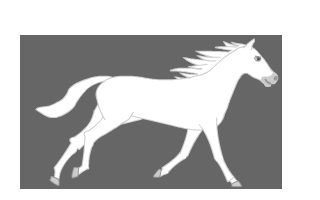
\includegraphics[width=3.5cm]{png/Horse_frame1.png}
  
\includegraphics[width=3.5cm]{png/Horse_frame2.png}
  
\includegraphics[width=3.5cm]{png/Horse_frame3.png}
  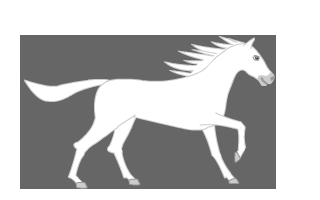
\includegraphics[width=3.5cm]{png/Horse_frame4.png}
\caption{\engt{4 frames to make a moving horse. The full animation: \href{http://en.wikipedia.org/wiki/File:Horse\_gif.gif}{Wikipedia Horse\_gif}} \nedt{4 frames om een bewegend paard te maken. De volledige animatie: \href{http://en.wikipedia.org/wiki/File:Horse\_gif.gif}{Wikipedia Horse\_gif}}}
\label{f:horse_movie}
\end{figure}

\eng{Let's put our idea in practice for the same effect we did with PWM: show a random color for a single second. As our LED cannot show as many colors as the full RGB range, we will limit the range from 256 gradations to 256/4=64 gradations. We express the scene in the Red, Green, Blue component in 64 gradations, and a duration to show a color:\newline
\textbf{scene = (red base 64, green base 64, blue base 64, duration)}.\newline
The action of this scene is to show a single red, green, blue color, so 
every frame is identical:
$$F= (\mbox{red, green, blue})$$
A subframe consists in showing this red, green or blue. Let's take red. If we show red, we will have a number from 0 to 64 to show. Let's call the number $R$, for example $R=35$. We said a subframe should be around 333$\mu$s. Let's take 64*5 = 320 $\mu$s. 

If the value of red is 64, we show red for 320$\mu$s, if the value is 0 we show red  0 $\mu$s in this subframe. So, for $R=35$, we show it 35*5=175$\mu$s.

The code to implement this is in Code \ref{c:l2_c}.
}

\ned{Laat ons dit indee in de praktijk brengen met hetzelfde effect dat we eerder via PWM deden: toon een willekeurige kleur voor een sekonde. Gezien de LED niet evenveel kleuren kan tonen als het volledige RGB spectrum, limiteren we de 256 gradaties in 256/4=64 gradaties. We drukken de scene uit in de Rood, Groen en Blauw component in 64 gradaties, en een duur om de kleur te tonen:\newline
\textbf{scene = (red base 64, green base 64, blue base 64, duration)}.\newline
De actie van deze scene is het tonen van een enkele rood, groen, blauw kleur, dus elke frame is identiek:
$$F= (\mbox{rood, groen, blauw}).$$
Een subframe bestaat in het tonen van rood, groen, of blauw. Laat ons rood nemen. We zullen een number van 0 tot 64 hebben voor rood. Laat ons dit nummer $R$ noemen, bevoorbeeld $R=35$. We hebben reeds gezegd dat de duur van het subframe rond de 333$\mu$s moet zijn. Laat ons 64*5=320 nemen als duur van het subframe. 

Als de waarde van rood 64 is, tonen we rood voor 320$\mu$s, als de waarde 0 is tonen we rood 0$\mu$s in dit subframe. Dus, voor $R=35$, tonen we het 35*5=175$\mu$s.

The code om dit te implementeren is in Code \ref{c:l2_c}.
}

\begin{code}\label{c:l2_c}
 \ \newline
\inputardfull{\string"../sketches/Fe_cube_02_RGB_frames/Fe_cube_02_RGB_frames.ino\string"}
\end{code}

\eng{The code seems quite complex, but is actually divided in two parts: shots or actions you create, and a generic part that decides when a new frame is needed, requests the new frame from the shot, and then starts up subframe cycles to show this specific frame for 40 ms. This last part will remain the same, if you feel up to it, you can try to understand it, but if not, no problem, it suffices to be able to write new shots.

So, let's go over the code. As always, we define first the pins we will use. Then the \ardo{setup()} function comes, that prepares the arduino. Nothing new there. 

Next, we have a function for our shot: a random color. This function has a specific signature that all our shots need to have:\newline
\textbf{ void random\_color(unsigned long framenr, int frame{$\lbrack$}3{$\rbrack$})}.\newline
So, a shot returns nothing. That is indicated with \ardo{void}. It needs two parameters:
the framenr of the shot, and a list of 3 integers: {int frame{$\lbrack$}3{$\rbrack$}}. The function will fill up this list with the frame to show. That is it! As our colors are values from 0 to 64, we use \ardo{random(65)}. To test you can indeed show all colors, instead of using random, change the code to see red, green, or blue. 

The following function defines our movie. The movie function definition seems very complicated. In reality it just indicates the movie function will return a shot function, like our random\_color above. Apart from this, the movie function is passed a variable \ardo{shotduration}, which must be set with how many milliseconds the shot must take. Internally, every time a shot is finished, this function \ardo{movie} will be called to obtain the next shot.

Below those two functions comes the internal loop to show a shot. This loop will call \ardo{movie} to obtain new shots, and will call the shot to obtain the frame to show. It will then take care of showing this frame for the frame duration (40ms). That's it.
}

\ned{De code ziet er complex uit, maar is eigenlijk verdeelt in twee delen: shots of acties die jij maakt, en een algemeen deel welke beslist wanneer een nieuw frame nodig is, dit frame opvraagt van de shot, en dan subframe cyclussen start om dit specifieke frame 40ms te tonen. Dit laatste deel zal niet meer wijzigen, als je wil kun je proberen het te verstaan, als niet, geen probleem, het volstaat in staat te zijn je eigen shots te schrijven.

Laat ons over de code gaan. Zoals steeds beginnen we met de pinnen aanduiden die we zullen gebruiken. Dan komt de  \ardo{setup()} functie, welke de arduino klaarmaakt. Niets nieuws dus.

Vervolgens hebben we de functie voor ons shot: een willekeurige kleur. Deze functie heeft een specifiek functievoorschrift die al onze shots zullen moeten hebben:\newline
\textbf{ void random\_color(unsigned long framenr, int frame{$\lbrack$}3{$\rbrack$})}.\newline
Dus, een shot geeft geen waarde terug. Dit duiden we aan met  \ardo{void}. Het heeft wel twee parameters nodig:
het framenummer van het shot, en een lijst van 3 integers: {int frame{[}3{]}}. De functie dient deze lijst op te vullen met het frame dat getoond moet worden. Dat is het! Gezien onze kleuren lopen van 0 tot 64, gebruiken we \ardo{random(65)}. Om te testen dat je alle kleuren kunt tonen, wijzig eens random in de waarde voor enkel rood, groen, of blauw. 

De volgende functie beschrijft onze film (\textit{movie} in het Engels). De functie definitie ziet er heel complex uit. In werkelijkheid duidt deze gewoon aan dat de \ardo{movie} functie een shot functie teruggeeft als waarde, zoals bevoorbeeld onze \ardo{random_color} functie van hierboven. Daarnaast krijgt de functie een variabele mee, \ardo{shotduration}, welke moet opgevuld worden met het aantal milliseconds de shot moet duren. De code zal telkens als een shot gedaan is, deze functie \ardo{movie} opnieuw oproepen om een volgend shot te bekomen.

Onder deze twee functies komt dan de interne arduino \ardo{loop} om een shot te tonen. Deze loop zal dus  \ardo{movie} oproepen om nieuwe shots te bekomen, en zal dan de shot oproepen om een frame nummer te bekomen. Het zal er dan voor zorgen dat deze frame getoond wordt voor de duur van een frame (40ms). Dat is het.
}
\subsection{\engt{Smooth transitions} \nedt{Gladde overhangeng}}

\eng{We now extend the previous code, and create a new shot, as example of how to add shots. This shot is a smooth transition from a first color to a next color.

The code for the shot, and the \ardo{movie} function can be found in Code \ref{c:l2_d}.
So this replaces the shot and the movie part of the previous section. 

Some remarks on the code. We divide the entire duration in frames, and calculate which one is needed. When we do the transition, we use blending of the two colors: this is a number between 0 and 1, call it $b$. We then mix begin and end color as: 
$$(1-b)\times \mbox{begincolor} + b \times \mbox{endcolor}.$$
So, if we start with $b=0$, we have the begincolor, and at $b=1$ we have the endcolor. 

When you divide two integers, the result is an integer, so we use the \ardo{float} function to change an integer into a float. Like this we find the blend between 0 and 1 for a specific frame number. Finally, our frame consists of colors which we denote as an integer between 0 and 64, so we apply the \ardo{round} function to convert the float to the nearest integer. For example \ardo{round(1.3)=1} and \ardo{round(1.6)=2}.
}

\ned{We breiden nu de vorige code uit, en maken een nieuw shot, als voorbeeld van hoe we shots kunnen toevoegen. Dit shot is een gladde overgang van een eerste kleur naar een andere kleur.

De code voor dit shot, en de \ardo{movie} functie die ze roept kun je vinden in  Code \ref{c:l2_d}. Dit vervant het shot en movie deel van de vorige sectie.

Enkele opmerkingen. We verdelen de volledige duur in frames, en berekenen welke we nodig hebben. Als we een transitie doen blenden we de twee kleuren: dat is een nummer tussen 0 en 1, noem het $b$. We mixen dan begin en eindkleur als:
$$(1-b)\times \mbox{beginkleur} + b \times \mbox{eindkleur}.$$
Als we dus starten met $b=0$, hebben we de beginkleur, en voor $b=1$ de eindkleur.

Als je twee gehele getallen deelt, is het resultaat opnieuw een geheel getal. Daarom gebruiken we de \ardo{float} functie om een geheel getal (integer) in een re\"eel getal (float) te veranderen. Zo vinden we de blend tussen 0 en 1 voor een specifieke frame. Maar, ons frame bestaat wel uit kleuren die we aanduiden met een getal tussen 0 en 64, daarom passen we de functie \ardo{round} to om de float te veranderen in de dichstbijgelegen integer. Bijvoorbeeld:  \ardo{round(1.3)=1} en \ardo{round(1.6)=2}.
}

\begin{code}\label{c:l2_d}
 \ \newline
\inputard{\string"../sketches/Fe_cube_02_RGB_smooth_trans/Fe_cube_02_RGB_smooth_trans.ino\string"}{47}{112}
\end{code}


\engo{\begin{doE}
      \textbf{Your shot!}. Make your own shot now. For example, blink the led always faster and faster.
      
      Tip: For example, if the shot is 60 seconds, and you start with a 2 second interval, you want to end with a 0.001 second interval. So, your interval could decrease linearly:
      $$y=2+\frac{0.001-2}{60} \mbox{time}$$

      Nicer: mix, this is blinking sequentially two different colors always faster. You should see them mix in front of you. Still nicer: mix red, green and blue amounts.
     \end{doE}
}
\nedo{\begin{doN}
      \textbf{Jouw shot}. Maak nu je eigen shot. Bevoorbeeld, knipper de led altijd maar sneller en sneller.
      
      Tip: Bevoorbeeld, als je shot 60 seconden is, en je start van een 2 seconden interval, en je wil eindigen met een 0.001 sekonden interval, dan moeten je intervallen lineair afnemen:
      $$y=2+\frac{0.001-2}{60} \mbox{tijd}$$

      Mooier: mengen, dit is twee kleuren afwisselend knipperen, en dit versnellen. Je zou de kleuren moeten zien vermengen. Nog mooier: rood, groen en blauw hoeveelheden mengen
     \end{doN}
}

\newpage
\section{\engt{Lesson 3: LED Cube Construction} \nedt{Les 3: LED Cube constructie}}

\subsection{\engt{Layout breadboard}  \nedt{Opstelling schakelbord}}

\eng{We have all the necessary basis to start with making our Fe Cube. We start with putting all components on the breadboard. Then we test it with a program which is our previous RGB LED sketch adapted to the cube. Only when we have verified all works will we start the actual construction.

So, put following components in front of you:
\begin{enumerate}
 \item Your breadboard
 \item 9 RGB-LED (we assume common kathode in the following)
 \item 3 NPN (2N3904 normally)
 \item 9 220 $\Omega$ resistors
 \item many wires.
\end{enumerate}
First, put the RGB-LED on the board, connect the color pins with each other via wires, and connect the common kathode via a resistor to another line, see Fig.~\ref{f:lesson3_bb1}.

Connect then the resistors to pins 1 to 9. These are the pins that will feed the LED. So for a common kathode, these pins on \ardo{HIGH} will make the LED burn. Put the 3 NPN on the board. The color wire goes to the Emittor side (+) of the NPN for common kathode LED. The Collector side (-) goes to the GND line of your breadboard. The GND line of the breadboard goes to a GND pin on the Arduino.

The Base leg of the NPN will control if the NPN junction is open or not. We will use pins 10, 11, 12 to control this. Your entire wiring should look like Fig.~\ref{f:lesson3_bb2}.
}

\ned{We hebben alles gezien om aan onze Fe Kubus te beginnen. We starten met alle componenten op het schakelbord te zetten. Dan testen we de schakeling met een programma die onze vorige RGB LED schets is aangepast voor de kubus. Alleen als we zeker zijn dat alles werkt zullen we de effectieve constructie doen.

Plaats dus de volgende componenten voor jou:
\begin{enumerate}
 \item Jouw schakelbord
 \item 9 RGB-LED (we veronderstellen gemeenschappelijke kathode in wat volgt)
 \item 3 NPN (2N3904 normaal)
 \item 9 220 $\Omega$ weerstanden
 \item veel draden.
\end{enumerate}
Begin met de RGB-LED op je bord te zetten, verbindt de kleurpinnen met elkaar via draden, en connecteer de gemeenschappelijke kathode via een weerstand naar een andere lijn op je bord, zie Fig.~\ref{f:lesson3_bb1}.

Verbind nu de weerstanden met pinnen 1 tot 9. Deze pinnen zullen de LED van stroom voorzien. Dus, voor een gemeenschappelijke kathode zullen we deze pinnen op \ardo{HIGH} zetten om de LED te doen branden. Plaats dan de 3 NPN op het bord. De draden van een kleur gaan naar de Emittor zijde (+) van de NPN voor gemeenschappelijke kathode LEDs. De Collector zijde (-) gaat naar de GND lijn op je schakelbord. Deze GND lijn gaat dan naar een GND pin op de Arduino.

Het Basis been van de NPN zal bepalen of de NPN junctie open is of niet. We zullen pinnen 10, 11, 12 gebruiken voor dit been. Je volledige schakeling zou er moeten uitzien als Fig.~\ref{f:lesson3_bb2}.
}

\begin{figure}
  \centering
  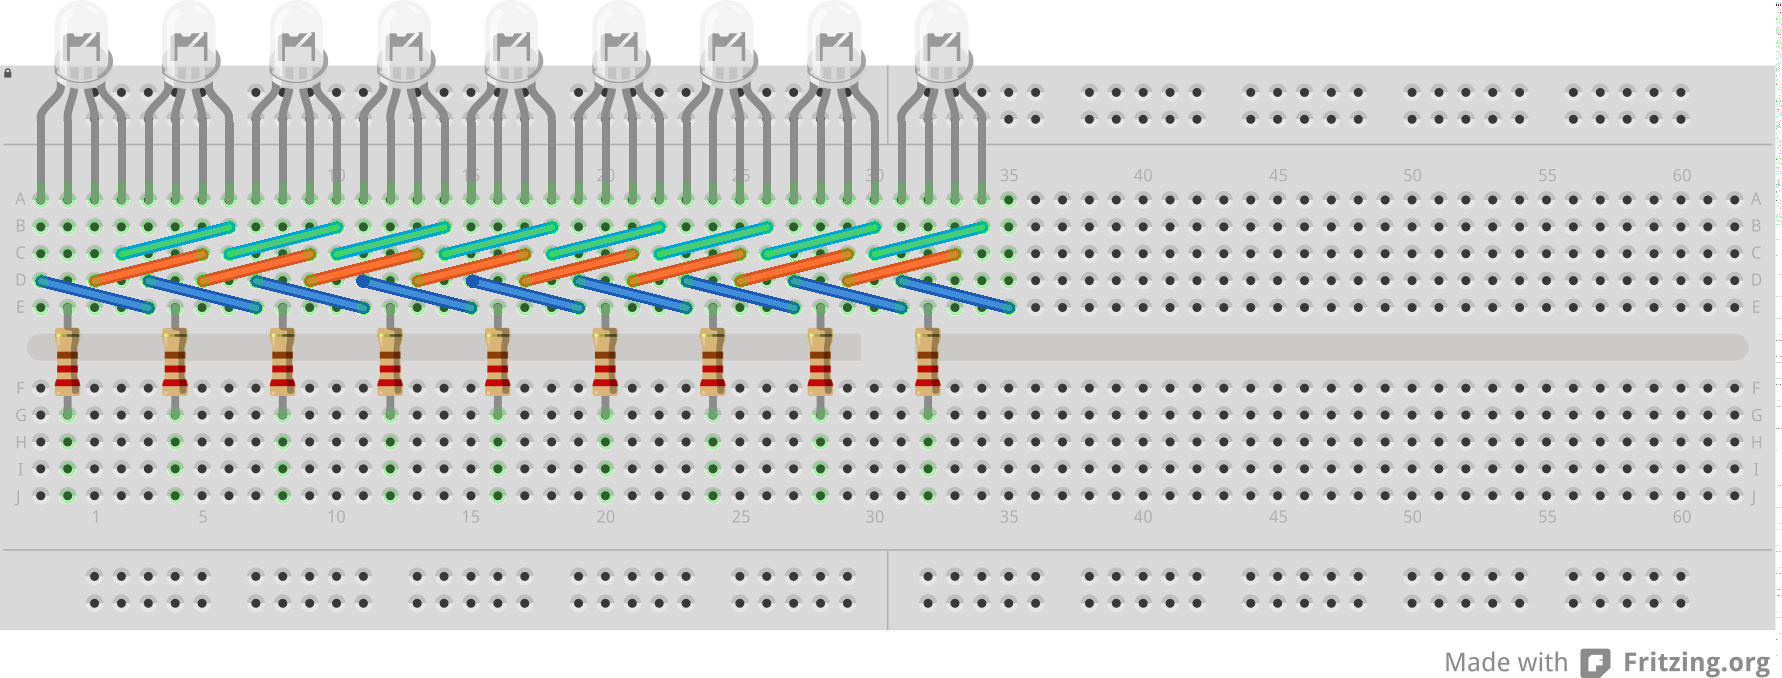
\includegraphics[width=11cm]{img/05_fecube_01_bb.png} 
\caption{\engt{Put the 9 LED on the board. Connect all equal colors to each other. The common kathode or anode goes with a 220 $\Omega$ resistor to a new line} \nedt{Plaats de 9 LED op het bord. Connecteer alle gelijke kleuren met elkaar. De gemeenschappelijke kathode of anode gaat met een 220 $\Omega$ weerstand naar een nieuwe lijn.}}
\label{f:lesson3_bb1}.
\end{figure}
%
\begin{figure}
  \centering
  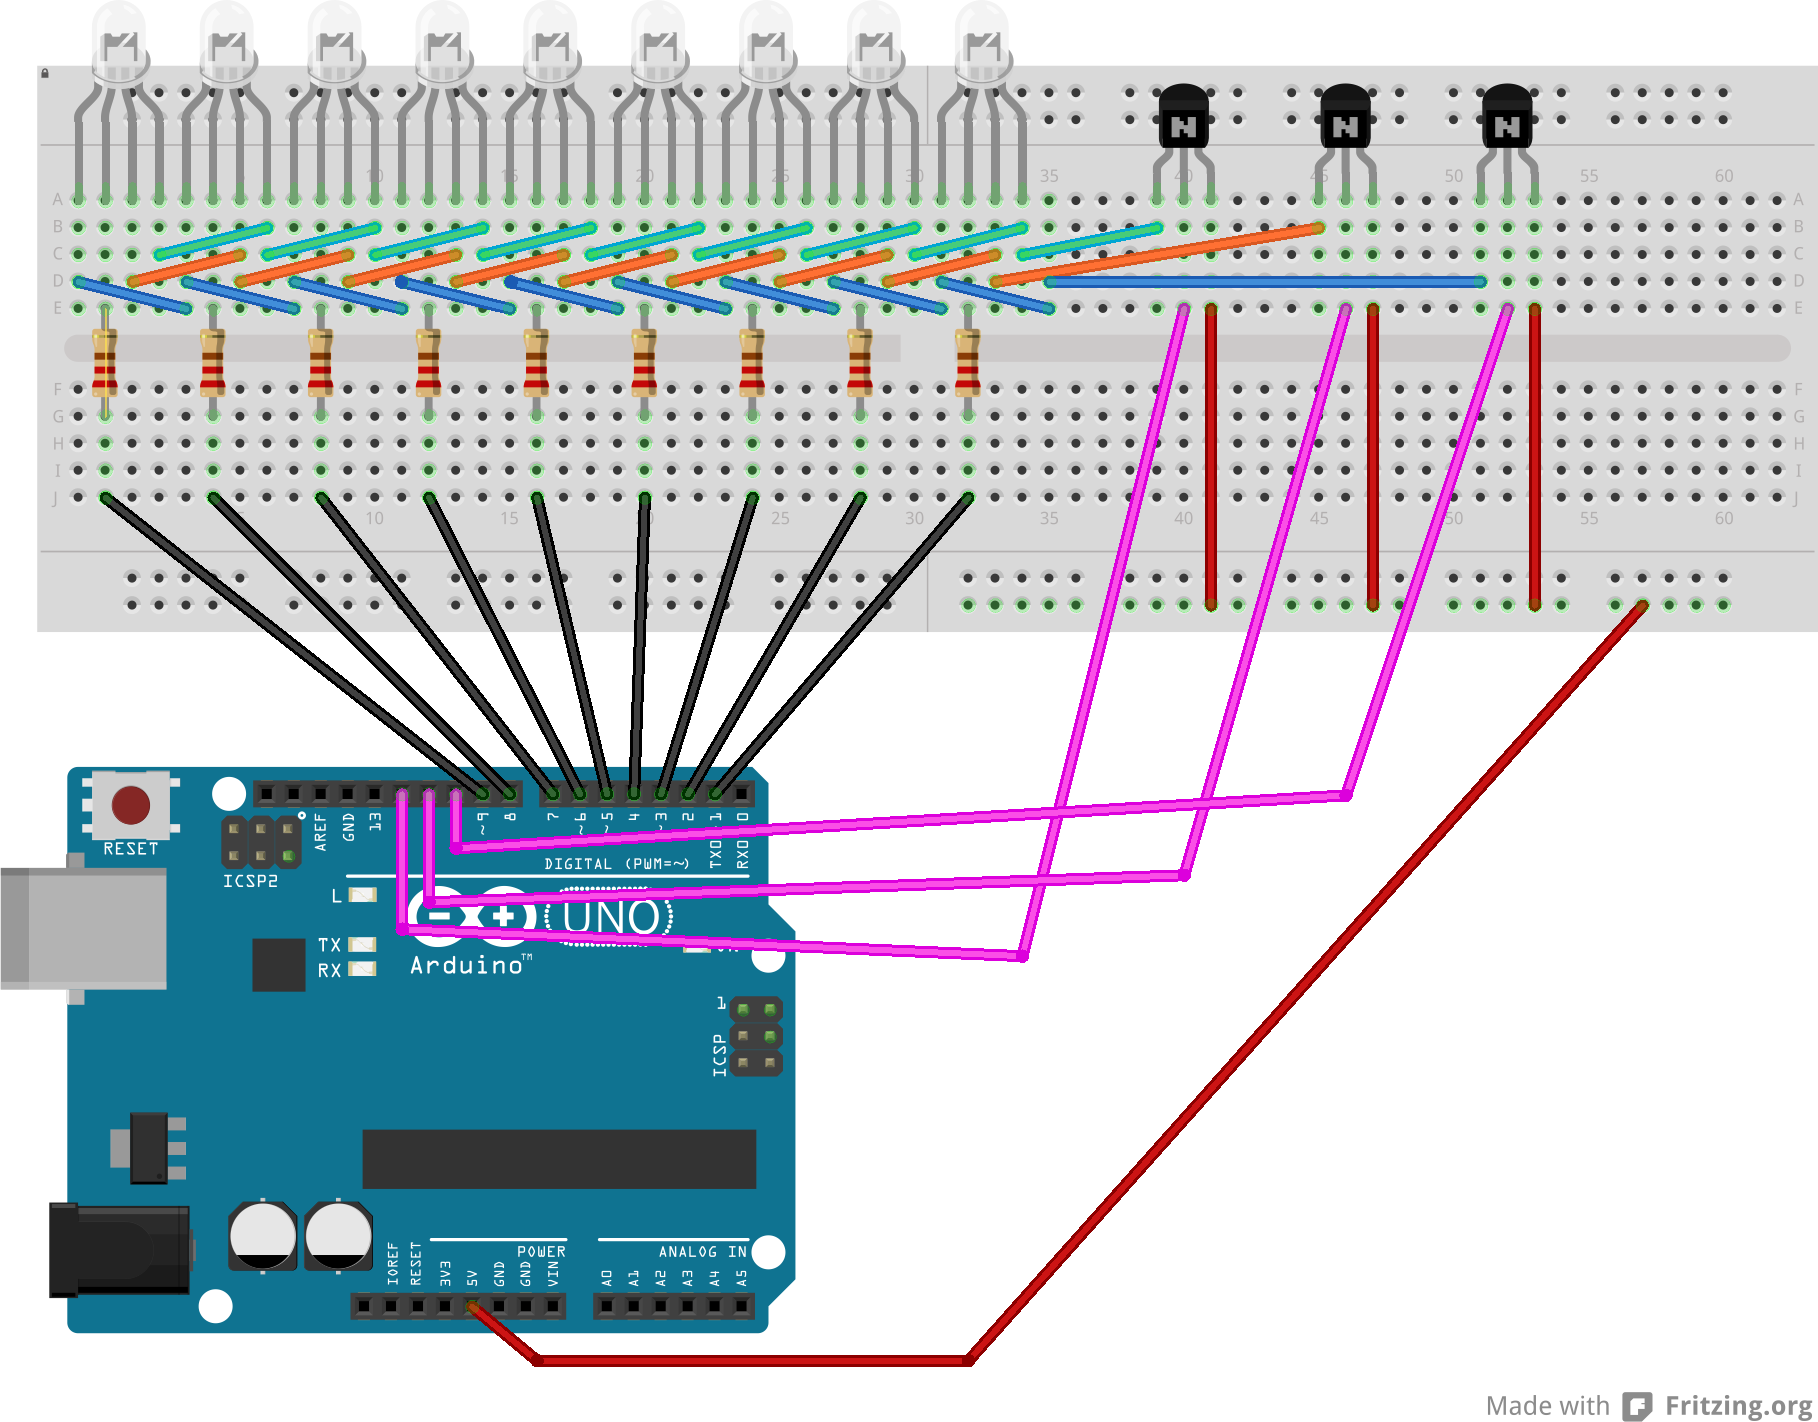
\includegraphics[width=11cm]{img/05_fecube_02_bb.png} 
\caption{\engt{Connect the resistors to pins 1 to 9. The colors go via an npn to the GND (kathode) or 5V (anode). Pins 10, 11, 12 go to the NPN to control the colors.} \nedt{Verbind de weerstanden met pinnen 1 tot 9. De kleuren gaan via een npn naar de GND (kathode) of 5V (anode). Pinnen 10, 11, 12 gaan naar de NPN om de kleuren te schakelen.}}
\label{f:lesson3_bb2}
\end{figure}


\subsection{\engt{Testing breadboard Fe Cube}  \nedt{Schakelbord Fe Cube uittesten}}

\eng{We will only verify we can make the breadboard Fe Cube work. For this we adapt our RGB sketches. We will make a movie showing 1 minute a random color, then 4 seconds red, then 4 seconds green, then 4 seconds blue, then smooth transitions for 1 minute.

This means we need all the shots we created for the RGB LED in the previous lesson, and need to create an adapted \ardo{movie} function to connect the shots as we want. We also need to change the start so that instead of only one led pin, we start up 9 led pins. 

The Code can be found in ...
}

\ned{TODO}

\section{\engt{Lesson 4: Fire up the LED Cube} \nedt{Les 4: De LED Cube gebruiken}}

\subsection{\engt{RGB Switching} \nedt{RGB Schakelen}}
\eng{You finished now constructing the cube. We need to test if all lights are working, as well if we can obtain the 3 root colors: red, green and blue.  So, based on the Arduino sketch for the single led, create a sketch that shows 1 second red, 1 second blue, and finally 1 second green, looping this sequence infinitely. 

Be ready to switch of the power quickly. If you have short circuits or other problems, LEDs can blow out! It is not a bad idea to test beforehand with a coin battery if you can power up the LEDs, but also here, connecting wrong pins can blow out the LED. 

Your code should look like the one in Code Fragment \ref{c:ledcube_rgb}.
}

\ned{TODO}

\begin{code}\label{c:ledcube_rgb}
 \ \newline
%\inputardfull{\string"sketches/Fe_cube_RGB_cube_test/Fe_cube_RGB_cube_test.ino\string"}
\end{code}

\eng{If things are not work, you have some extra soldering to do: replace a blown out LED, make connections stronger, ... . Don't give up now. These are the last construction problems of your led cube.}
\ned{TODO}

\subsection{\engt{Naming pins} \nedt{Pinnen benoemen}}
\eng{In our previous script, we had ledR, ledG, ledB, which are easy to understand names. The other leds are called from 1 to 9. This is not very helpfull if you want to program certain light effects. So, let's give them better names. We have a top layer (T), and a bottom (B) layer, and a single LED in the middle. Then we can divide the cube in a left (L) and right (R), and in a front (F) and an aft (A). So, let's call the LEDs:
\begin{enumerate}
\item ledTLF
\item ledTLA
\item ledTRF
\item ledTRA
\item ledBLF
\item ledBLA
\item ledBRF
\item ledBRA
\item ledMID
\end{enumerate}

Next, test that every LED is correctly wired by cycling over every single led one after the other for 1 seconds. Define an order of switching the led, for example, in a snake like manner.

Our code is given in Code \ref{c:ledcube_snake}
}

\ned{TODO}

\begin{code}\label{c:ledcube_snake}
 \ \newline
%\inputardfull{\string"sketches/Fe_cube_RGB_cube_test2/Fe_cube_RGB_cube_test2.ino\string"}
\end{code}


\subsection{Smooth Transitions - Mooie overgangen} 
\eng{Now that we have verified we can control every aspect of our Fe Cube, we convert our Mixing colors script to now drive the cube. So, instead of one LED, we will be having 9 leds that smoothly go from one random color to the next. This will produce more light than our single LED on our test board.}

\ned{
TODO}


\begin{code}\label{c:ledcube_smooth}
 \ \newline
%\inputardfull{\string"sketches/Fe_cube_04_common_kathodeRGB_cube_smoothrandom/Fe_cube_04_common_kathodeRGB_cube_smoothrandom.ino\string"}
\end{code}

\end{Parallel}

\end{document}
